\documentclass[a4paper,oneside,12pt]{ThesisStyle}

\usepackage{amsmath,amssymb}             % AMS Math
\usepackage{bbm}
\usepackage[utf8]{inputenc}
\usepackage[T1]{fontenc}
\usepackage[ngerman]{babel}
\usepackage[left=1.0in,right=3.5cm,top=0.4in,bottom=1.1in,includefoot,includehead,headheight=13.6pt]{geometry}
\renewcommand{\baselinestretch}{1.05}

% Table of contents for each chapter

\usepackage[nottoc, notlof, notlot]{tocbibind}
\usepackage[german]{minitoc}
\setcounter{minitocdepth}{2}
\mtcindent=15pt
% Use \minitoc where to put a table of contents

\usepackage{aecompl}

% Glossary / list of abbreviations [Abk�rzungsverzeichnes]

\usepackage[intoc]{nomencl}
\let\abvz\nomenclature
\renewcommand{\nomname}{Abk{\"u}rzungsverzeichnes}
\setlength{\nomlabelwidth}{.25\hsize}
\renewcommand{\nomlabel}[1]{#1\dotfill}
\setlength{\nomitemsep}{-\parsep}

\makenomenclature

% include matlab code into Latex
\usepackage[framed]{mcode}
% My pdf code

\usepackage{ifpdf}

\ifpdf
  \usepackage[pdftex]{graphicx}
  \DeclareGraphicsExtensions{.png,.pdf,.jpg}
  \usepackage[a4paper,pagebackref,hyperindex=true]{hyperref}
\else
  \usepackage{graphicx}
  \DeclareGraphicsExtensions{.ps,.eps}
  \usepackage[a4paper,dvipdfm,pagebackref,hyperindex=true]{hyperref}
\fi

\graphicspath{{.}{images/}}

% Links in pdf
\usepackage{color}
\definecolor{linkcol}{rgb}{0,0,0.4} 
\definecolor{citecol}{rgb}{0.5,0,0} 

% Change this to change the informations included in the pdf file

% See hyperref documentation for information on those parameters

\hypersetup
{
bookmarksopen=true,
pdftitle="Realisation und Simulation einer Kaeltelast mit Kaeltespeicher im Energieversorgungsnetz",
pdfauthor="Juri STEBLAU",
pdfsubject="Creation of refrigerator simulation with MATLAB", %subject of the document
%pdftoolbar=false, % toolbar hidden
pdfmenubar=true, %menubar shown
pdfhighlight=/O, %effect of clicking on a link
colorlinks=true, %couleurs sur les liens hypertextes
pdfpagemode=None, %aucun mode de page
pdfpagelayout=SinglePage, %ouverture en simple page
pdffitwindow=true, %pages ouvertes entierement dans toute la fenetre
linkcolor=linkcol, %couleur des liens hypertextes internes
citecolor=citecol, %couleur des liens pour les citations
urlcolor=linkcol %couleur des liens pour les url
}

% definitions.
% -------------------

\setcounter{secnumdepth}{3}
\setcounter{tocdepth}{2}

% Some useful commands and shortcut for maths:  partial derivative and stuff

\newcommand{\pd}[2]{\frac{\partial #1}{\partial #2}}
\def\abs{\operatorname{abs}}
\def\argmax{\operatornamewithlimits{arg\,max}}
\def\argmin{\operatornamewithlimits{arg\,min}}
\def\diag{\operatorname{Diag}}
\newcommand{\eqRef}[1]{(\ref{#1})}
\usepackage{rotating}                    % Sideways of figures & tables
%\usepackage{bibunits}
%\usepackage[sectionbib]{chapterbib}          % Cross-reference package (Natural BiB)
%\usepackage{natbib}                  % Put References at the end of each chapter
                                         % Do not put 'sectionbib' option here.
                                         % Sectionbib option in 'natbib' will do.
\usepackage{fancyhdr}                    % Fancy Header and Footer

% \usepackage{txfonts}                     % Public Times New Roman text & math font
  
%%% Fancy Header %%%%%%%%%%%%%%%%%%%%%%%%%%%%%%%%%%%%%%%%%%%%%%%%%%%%%%%%%%%%%%%%%%
% Fancy Header Style Options

\pagestyle{fancy}                       % Sets fancy header and footer
\fancyfoot{}                            % Delete current footer settings

%\renewcommand{\chaptermark}[1]{         % Lower Case Chapter marker style
%  \markboth{\chaptername\ \thechapter.\ #1}}{}} %

%\renewcommand{\sectionmark}[1]{         % Lower case Section marker style
%  \markright{\thesection.\ #1}}         %

\fancyhead[LE,RO]{\bfseries\thepage}    % Page number (boldface) in left on even
% pages and right on odd pages
\fancyhead[RE]{\bfseries\nouppercase{\leftmark}}      % Chapter in the right on even pages
\fancyhead[LO]{\bfseries\nouppercase{\rightmark}}     % Section in the left on odd pages

\let\headruleORIG\headrule
\renewcommand{\headrule}{\color{black} \headruleORIG}
\renewcommand{\headrulewidth}{1.0pt}
\usepackage{colortbl}
\arrayrulecolor{black}

\fancypagestyle{plain}{
  \fancyhead{}
  \fancyfoot{}
  \renewcommand{\headrulewidth}{0pt}
}

\usepackage{algorithm}
\usepackage[noend]{algorithmic}

%%% Clear Header %%%%%%%%%%%%%%%%%%%%%%%%%%%%%%%%%%%%%%%%%%%%%%%%%%%%%%%%%%%%%%%%%%
% Clear Header Style on the Last Empty Odd pages
\makeatletter

\def\cleardoublepage{\clearpage\if@twoside \ifodd\c@page\else%
  \hbox{}%
  \thispagestyle{empty}%              % Empty header styles
  \newpage%
  \if@twocolumn\hbox{}\newpage\fi\fi\fi}

\makeatother
 
%%%%%%%%%%%%%%%%%%%%%%%%%%%%%%%%%%%%%%%%%%%%%%%%%%%%%%%%%%%%%%%%%%%%%%%%%%%%%%% 
% Prints your review date and 'Draft Version' (From Josullvn, CS, CMU)
\newcommand{\reviewtimetoday}[2]{\special{!userdict begin
    /bop-hook{gsave 20 710 translate 45 rotate 0.8 setgray
      /Times-Roman findfont 12 scalefont setfont 0 0   moveto (#1) show
      0 -12 moveto (#2) show grestore}def end}}
% You can turn on or off this option.
% \reviewtimetoday{\today}{Draft Version}
%%%%%%%%%%%%%%%%%%%%%%%%%%%%%%%%%%%%%%%%%%%%%%%%%%%%%%%%%%%%%%%%%%%%%%%%%%%%%%% 

%%%%%%%%%%%%%%%%%%%%%%%%%%%%%%%%%%%%%%%%%%%%%%%%%%%%%%%%%%%%%%%%%%%%%%%%%%%%%%%%%%%
% Matlab for shortc
\newcommand{\matlab}{\textsc{Matlab\textsuperscript{\textsf{\textregistered}}}\,}
\newcommand{\matref}[1]{\matlab-Code~\ref{#1}}
%\renewcommand{\todo}{\todo$\,$}
%%%%%%%%%%%%%%%%%%%%%%%%%%%%%%%%%%%%%%%%%%%%%%%%%%%%%%%%%%%%%%%%%%%%%%%%%%%%%%%%%%%


\newenvironment{maxime}[1]
{
\vspace*{0cm}
\hfill
\begin{minipage}{0.5\textwidth}%
%\rule[0.5ex]{\textwidth}{0.1mm}\\%
\hrulefill $\:$ {\bf #1}\\
%\vspace*{-0.25cm}
\it 
}%
{%

\hrulefill
\vspace*{0.5cm}%
\end{minipage}
}

\let\minitocORIG\minitoc
\renewcommand{\minitoc}{\minitocORIG \vspace{1.5em}}

\usepackage{multirow}
\usepackage{slashbox}

\newenvironment{bulletList}%
{ \begin{list}%
	{$\bullet$}%
	{\setlength{\labelwidth}{25pt}%
	 \setlength{\leftmargin}{30pt}%
	 \setlength{\itemsep}{\parsep}}}%
{ \end{list} }

\newtheorem{definition}{D�finition}
\renewcommand{\epsilon}{\varepsilon}

% centered page environment

\newenvironment{vcenterpage}
{\newpage\vspace*{\fill}\thispagestyle{empty}\renewcommand{\headrulewidth}{0pt}}
{\vspace*{\fill}}

% t_odo shit
\usepackage[textwidth=3.2cm]{todonotes}


%% i try \newfloat
%\floatstyle{plain}
%\usepackage{float}
%\newfloat{macode}{h}{mcd}[chapter]
%\floatname{macode}{Quellcode}
%
%% i try table of list of ..
%\usepackage{tocloft}
%\newcommand{\listmacode}{List of Quellcodes}
%\newlistof{mascode}{ex}{\listmacode}
%\newcommand{\mascode}[1]{%
%\refstepcounter{mascode}
%\par\noident\textbf{mascode \qqcode. #1}
%\addcontentsline{exp}{qcode}
%{\protect\number{\thechapter. \qqcode}#1}\par}


%%%%%%%%%%%%%%%%%%%%%%%%%%%%%%%%%%%%%%%%%%%%%%%%%%%%%%%%%%%%%%%%%%%%%%%%%%%%%%%%%%%%%%%%%%%%%%%%%%%%%%%%%%%%%%%%%%%%%%%%%%%%
% bebtex my try
\usepackage[nospace]{cite}
%%%%%%%%%%%%%%%%%%%%%%%%%%%%%%%%%%%%%%%%%%%%%%%%%%%%%%%%%%%%%%%%%%%%%%%%%%%%%%%%%%%%%%%%%%%%%%%%%%%%%%%%%%%%%%%%%%%%%%%%%%%%
\usepackage{multibib}
%%%%%%%%%%%%%%%%%%%%%%%%%%%%%%%%%%%%%%%%%%%%%%%%%%%%%%%%%%%%%%%%%%%%%%%%%%%%%%%%%%%%%%%%%%%%%%%%%%%%%%%%%%%%%%%%%%%%%%%%%%%%
% remember footnote and refer to that many times!
\newcommand{\footnoteremember}[2]{%
	\footnote{#2}%
	\newcounter{#1}%
	\setcounter{#1}{\value{footnote}}%
}
\newcommand{\footnoterecall}[1]{%
	\footnotemark[\value{#1}]%
}
%%%%%%%%%%%%%%%%%%%%%%%%%%%%%%%%%%%%%%%%%%%%%%%%%%%%%%%%%%%%%%%%%%%%%%%%%%%%%%%%%%%%%%%%%%%%%%%%%%%%%%%%%%%%%%%%%%%%%%%%%%%%%
\usepackage[ngerman]{cleveref}
%%%%%%%%%%%%%%%%%%%%%%%%%%%%%%%%%%%%%%%%%%%%%%%%%%%%%%%%%%%%%%%%%%%%%%%%%%%%%%%%%%%%%%%%%%%%%%%%%%%%%%%%%%%%%%%%%%%%%%%%%%%%%
\setcounter{secnumdepth}{5}
%%%%%%%%%%%%%%%%%%%%%%%%%%%%%%%%%%%%%%%%%%%%%%%%%%%%%%%%%%%%%%%%%%%%%%%%%%%%%%%%%%%%%%%%%%%%%%%%%%%%%%%%%%%%%%%%%%%%%%%%%%%%%
\newcommand{\pinstall}{\dot{Q}_0^)}%
%%%%%%%%%%%%%%%%%%%%%%%%%%%%%%%%%%%%%%%%%%%%%%%%%%%%%%%%%%%%%%%%%%%%%%%%%%%%%%%%%%%%%%%%%%%%%%%%%%%%%%%%%%%%%%%%%%%%%%%%%%%%%
\newcommand{\ptrans}{\dot{Q}_{Tr}}%
%%%%%%%%%%%%%%%%%%%%%%%%%%%%%%%%%%%%%%%%%%%%%%%%%%%%%%%%%%%%%%%%%%%%%%%%%%%%%%%%%%%%%%%%%%%%%%%%%%%%%%%%%%%%%%%%%%%%%%%%%%%%%
\newcommand{\pkalt}{\dot{Q}_{0}}%
%%%%%%%%%%%%%%%%%%%%%%%%%%%%%%%%%%%%%%%%%%%%%%%%%%%%%%%%%%%%%%%%%%%%%%%%%%%%%%%%%%%%%%%%%%%%%%%%%%%%%%%%%%%%%%%%%%%%%%%%%%%%%
\newcommand{\emehr}{Q_{mehr}}%
%%%%%%%%%%%%%%%%%%%%%%%%%%%%%%%%%%%%%%%%%%%%%%%%%%%%%%%%%%%%%%%%%%%%%%%%%%%%%%%%%%%%%%%%%%%%%%%%%%%%%%%%%%%%%%%%%%%%%%%%%%%%%
\newcommand{\pmehr}{\dot{Q}_{mehr}}%
%%%%%%%%%%%%%%%%%%%%%%%%%%%%%%%%%%%%%%%%%%%%%%%%%%%%%%%%%%%%%%%%%%%%%%%%%%%%%%%%%%%%%%%%%%%%%%%%%%%%%%%%%%%%%%%%%%%%%%%%%%%%%
\newcommand{\lmehr}{{W}_{mehr}}%
%%%%%%%%%%%%%%%%%%%%%%%%%%%%%%%%%%%%%%%%%%%%%%%%%%%%%%%%%%%%%%%%%%%%%%%%%%%%%%%%%%%%%%%%%%%%%%%%%%%%%%%%%%%%%%%%%%%%%%%%%%%%%
\newcommand{\lverd}{{W}_{Verd_{24}}}%
%%%%%%%%%%%%%%%%%%%%%%%%%%%%%%%%%%%%%%%%%%%%%%%%%%%%%%%%%%%%%%%%%%%%%%%%%%%%%%%%%%%%%%%%%%%%%%%%%%%%%%%%%%%%%%%%%%%%%%%%%%%%%
\newcommand{\lspez}{{W}_{spez_{24}}}%
%%%%%%%%%%%%%%%%%%%%%%%%%%%%%%%%%%%%%%%%%%%%%%%%%%%%%%%%%%%%%%%%%%%%%%%%%%%%%%%%%%%%%%%%%%%%%%%%%%%%%%%%%%%%%%%%%%%%%%%%%%%%%
\newcommand{\pnacht}{\dot{Q}_{Nacht}}%
%%%%%%%%%%%%%%%%%%%%%%%%%%%%%%%%%%%%%%%%%%%%%%%%%%%%%%%%%%%%%%%%%%%%%%%%%%%%%%%%%%%%%%%%%%%%%%%%%%%%%%%%%%%%%%%%%%%%%%%%%%%%%
\newcommand{\ptag}{\dot{Q}_{Tag}}%



%%%Uml sequence diagrams
%\usepackage{tikz}
%%\usetikzlibrary{arrows} % for pgf-umsld
%\usetikzlibrary{arrows,shadows} % for pgf-umsld
%\bususepackage[underline=true, rounded corners=false]{pgf-umlsd}


\begin{document}

\begin{titlepage}
	\begin{figure}[!ht]
		\parbox{0.5\textwidth}{
\includegraphics[height=2.4cm]{Title_Page/TU-logo_rot}}
		\qquad
		\begin{minipage}{0.4\textwidth}
			\begin{flushright}
				
\includegraphics[height=2.41cm]{Title_Page/sense}
			\end{flushright}
		\end{minipage}
	\end{figure}
	\begin{center}
		\vspace*{0.5cm}
		\noindent {\large \textbf{TECHNISCHE UNIVERSITÄT BERLIN}}\\
		\vspace*{0.3cm}
		\noindent {\large \textbf{Fachgebiet Energieversorgungsnetz und Integration Erneuerbarer Energien}}\\
		\vspace*{2.8cm}
		\noindent {\large  \textbf{STUDIENARBEIT}}\\
		\vspace*{1.0cm}
		\noindent {\huge \textbf{Objektorientierte Implementierung}}\\
		\vspace*{0.1cm}
		\noindent {\huge \textbf{und Simulation}}\\
		\vspace*{0.3cm}
		\noindent {\huge \textbf{einer Kältelast mit Kältespeicher}}\\
		\vspace*{0.05cm}
		\noindent {\Huge \textbf{im Energieversorgungsnetz}}\\
		\vspace*{1.8cm}
		\noindent \large vorgelegt von Juri \textsc{Steblau}\\
		\noindent \large Matr.-Nr: \textsc{300244}\\
		\vspace*{0.8cm}
		\noindent \large \today \\
		\vspace*{1.5cm}
	\end{center}
	\noindent \large \textbf{Korrektoren:} \\
	\begin{center}
		\noindent \large
		\begin{tabular}{llcl}
			\text{Advisor:} 	& Dipl.-Ing. 	Felix \textsc{Klein} 	& - & (TU-Berlin)\\
			\text{Examinator:} 	& Prof.Dr.-Ing. Kai \textsc{Strunz} 	& - & (TU-Berlin)\\
		\end{tabular}
	\end{center}
\setcounter{page}{0}
\end{titlepage}
\sloppy

\titlepage


\dominitoc

\pagenumbering{roman}

\cleardoublepage

\cleardoublepage
\begin{vcenterpage}
	\noindent\rule[2pt]{\textwidth}{0.5pt}
	\begin{center}
		{\large\textbf{Realisation und Simulation einer K\"altelast mit K\"altespeicher im Energieversorgungsnetz}}
	\end{center}
	\noindent\rule[2pt]{\textwidth}{0.5pt}
	{\large\textbf{Abstract:}}
	Hier bitte am Ende der Arbeit auf english die kurze Inhaltsangabe schreiben. \todo[caption={Abstract nicht da},
	color=green!30, inline]{ Hier muss noch ein Abstract rein !!!AM ENDE!!!}
	{\large\textbf{Keywords:}}
	Möglicherweise in Englisch! Fuck!\\
	\noindent\rule[2pt]{\textwidth}{0.5pt}
\end{vcenterpage}



\listoftodos
\tableofcontents
\listoffigures
\mtcaddchapter[Abbildungsverzeichnis] % damit wird eine Eintrag im Inhaltsverzeichniss erzeugt.
\listoftables
\mtcaddchapter[Tabellenverzeichnis]
\lstlistoflistings
\mtcaddchapter[\matlab-Code Verzeichnis]
\printnomenclature % to get this toc! makeindex hauptdokument.nlo -s nomencl.ist -o hauptdokument.nls
\mtcfixglossary[chapter] % solve the conflict of \minitoc and \nomencl

\mainmatter % maindocument whit arabic numbers

\chapter{Einleitung}
\label{chap:einleitung}

%%%%%%%%%%%%%%%%%%%%%%%%%%%%%%%%%%%%%%%%%%%%%%%%%%%%%%%
%%%%%%%%%%%%%%%%%%%%%%%%%%%%%%%%%%%%%%%%%%%%%%%%%%%%%%%
%%%%%%%%%%%%%%%%%%%%%%%%%%%%%%%%%%%%%%%%%%%%%%%%%%%%%%%
%\section*{Studiere DAS} \todo{dont forget to delete!}
Die Einleitung ist der wichtigste Textabschnitt einer Hochschularbeit – und zwar gleichgültig, ob es sich um eine Diplomarbeit,
eine Bachelorthesis oder eine Staatsexamensarbeit handelt. Hier wird der Leser ins Thema eingeführt, hier wird die Fragestellung
formuliert, und hier werden die methodischen Grundsatzentscheidungen getroffen.

Tipp: Man sollte die Einleitung, auch wenn das sogar von Prüferseite geäußert wird, nicht zum Schluss schreiben, sondern sie vorab
verfassen und sie während der Niederschrift als Arbeitsinstrument verwenden. Denn hieran – und nur hieran – zeigt sich, ob das
Untersuchungsvorhaben klappt. Häufig zeigt sich auch, weshalb es nicht so gut klappt.

All das weiß auch der Prüfer. Daher steht im Grunde die Note schon nach der Lektüre der Einleitung fest – zumindest wird es
schwierig sein, den Prüfer davon zu überzeugen, dass es sich doch um eine gute Arbeit handelt, wenn die Einleitung misslungen ist.
Aber wie schreibt man nun eine gute Einleitung? Im Folgenden einige grundlegende Hinweise:

Hilfreich ist eine Aufteilung in vier Teile, die sinnvoll aufeinander aufbauen. Das heißt nicht, dass es nicht auch andere
Möglichkeiten gibt, aber so funktioniert es mit Sicherheit – bei jedem Thema.  Das vorgeschlagene Schema sieht wie folgt aus:

\begin{enumerate}
	\item Hinführung (2 Absätze); diese besteht im Idealfall aus dem
		\begin{enumerate}
			\item Einstieg (etwas, was an die allgemeine Erfahrung anknüpft und unmittelbar ersichtlich ist) und
			\item einem weiteren Absatz, in dem – ausgehend vom Einstieg – auf das eigentliche Thema fokussiert wird.
		\end{enumerate}
		In einer Arbeit über Online-Marketing mit Facebook beispielsweise würde es im 1. Absatz um Online-Marketing allgemein gehen und im 2. Absatz
		auf die besonderen Anforderungen im Zusammenhang mit Facebook verwiesen. (Kontrollfrage: „Worum geht es hier?“)

	\item Fragestellung (1 Satz), auch als Problemstellung oder Forschungsfrage bezeichnet. Dabei handelt es sich im
		Idealfall tatsächlich nur um einen Satz oder einen Fragesatz. Die Fragestellung muss sich organisch aus dem 2. Absatz der Hinführung
		ableiten lassen. Im Idealfall ergibt sich für den Leser selbst angesichts des bisher Vermittelten an exakt dieser Stelle eine Frage, die er
		dann vom Verfasser bzw. der Verfasserin
		formuliert bekommt. Damit einher geht die Vorgabe, dass die Fragestellung wirklich nur exakt eine einzige Frage bzw. ein Forschungsproblem
		betrifft, nicht zwei oder drei. Wenn das passiert, hat man schon an dieser Stelle etwas falsch gemacht.  (Kontrollfrage: „Was ist das
		Problem?“)
	\item Operationalisierung der Fragestellung (3 bis 4 Sätze); dabei wird die Frage beantwortet, welche inhaltlichen und methodischen Aspekte im
		Zusammenhang mit der Klärung der Forschungsfrage wichtig sind. Dabei dürfen dann durchaus weiterführende Fragen gestellt oder Hypothesen
		formuliert werden, die sich aber wiederum
		auf die zentrale Fragestellung zurückführen lassen müssen. (Kontrollfragen: „Welche Überlegungen sind damit verknüpft? Was brauche ich, um
		die Forschungsfrage zu beantworten?“)
	\item Untersuchungsverlauf (pro Kapitel ein – kurzer – Absatz mit Verweis auf die Kapitelnummer); hier wird geklärt, was Inhalt der einzelnen
		Kapitel ist. Neue inhaltliche oder methodische Aspekte sollten hier nicht mehr vorkommen, hier geht es nur noch um das Wie, nicht mehr um
		das Was. (Kontrollfrage: „Wie wird
		vorgegangen?“)
\end{enumerate}

Hinweis: Die Schritte 3 und 4 werden häufig vermischt, oder die Operationalisierung unterbleibt ganz. Wir möchten nochmals deutlich
darauf hinweisen, dass die inhaltlichen, vor allem aber die methodischen und strukturellen Überlegungen in Bezug auf die
Fragestellung ein unverzichtbares Instrument sind, um die grundlegenden Zusammenhänge der Untersuchung zu klären. Demgegenüber
dient der Untersuchungsverlauf lediglich dazu, die Überlegungen im Hinblick auf die Gliederung in eine sinnvolle Abfolge zu
bringen.

Wie gesagt, dieses Schema funktioniert mit jedem Thema – wenn nicht, deutet das eher darauf hin, dass mit dem Thema etwas nicht
stimmt. Konkrete Fragen dazu beantworten wir gern im o:T-Forum. Ansonsten lässt sich auch im Rahmen einer Kurzberatung klären, ob
die Einleitung schlüssig ist. Dazu ist keine Beauftragung eines Lektorats notwendig.

% Don't forget to delete this!!!!

%%%%%%%%%%%%%%%%%%%%%%%%%%%%%%%%%%%%%%%%%%%%%%%%%%%%%%%
%%%%%%%%%%%%%%%%%%%%%%%%%%%%%%%%%%%%%%%%%%%%%%%%%%%%%%%
%%%%%%%%%%%%%%%%%%%%%%%%%%%%%%%%%%%%%%%%%%%%%%%%%%%%%%%
Die\todo{Einleitung mehrfach durchlesen!} Erforschung der Ursachen und der
Folgen des Klimawandels, die wachsende Schwierigkeit bei der Bereitstellung der
konventionellen Energien, die Neubewertung der Risiken und technischen Mitteln
bei der Endlagerung von Abfällen der Atomindustrie, die besorgniserregende
Erkenntnis der bisherigen Fehlbewertung der Atomsicherheit
\textcolor{red}{werden mit Gewissheit} die politisch beschlossene Förderung der
erneuerbaren Energien zu einer grundlegenden Energieform in den kommenden Jahren
in Deutschland und in Europa forcieren.\todo{Reicht so? Guck bitte nach oben.}

Der Umstieg auf alternative Energien ist mit einigen\todo{Bewertung
einfügen.}$\,$ Problemen verbunden. An einigen Orten ist der Einsatz dieser
Technik aus politischer, technischer, ökonomischer oder ökologischer Sicht nicht
möglich. Darum weichen oft die Stromerzeugung und der Strombedarf zeitlich und
räumlich voneinander ab. Windkraft im Meer, Wasserkraft in den Bergen,
Sonnenkraft in dem Süden, Geothermie in Island\todo{Der Satz ist scheiße,
umschreiben.}, Biomasse Land. Es ist auch eine Tatsache, dass nur ein Teil der
erneuerbaren Energien direkt vom Menschen beeinflusst werden kann. Besonders die
Menge der durch Sonne und Wind gewonnenen Energie schwankt abhängig von der
Wetterlage. Die Integration dieser Energie in Netz führt zur erhöhten
Bereitstellung an Regelenergie. Hauptsächlich wird diese Herausforderung durch
übermäßige Belastung der zur Ausregelung geeigneten konventionellen thermischen
Kraftwerke gelöst. Durch den regelungsbedingten ineffizienten Teillastbetrieb
und wiederholte An- und Abfahrvorgänge sinkt der Wirkungsgrad und ein höherer
Verschleiß der ist die Folge. Aus langfristiger Sicht wird
jedoch\todo[color=red!70,inline]{Das am Ende zur Ende schreiben} eine
Investition in Lastmanagement und in Energiespeicher unentbehrlich sein.

Brückentechnologien nicht sicher. Politischer Druck wächst. 


\chapter{Theorie}
\label{chap:theorie}
\minitoc

%%%%%%%%%%%%%%%%%%%%%%%%%%%%%%%%%%%%%%%%%%%%%%%%%%%%%%%%%%%%%%%%%%%%%%%%%%%%%%%%
%%%%%%%%%%%%%%%%%%%%%%%%%%%%%%%%%%%%%%%%%%%%%%%%%%%%%%%%%%%%%%%%%%%%%%%%%%%%%%%%

\section{Erneuerbare Energien im Energieversorgungsnetz}

Die Erneuerbaren Energien \"ubernehmen in Deutschland mit jedem Jahr einen
gr\"o\ss eren Anteil an der Elektrizit\"atsversorgung. Mehr als die H\"alfte der
Erneuerbaren Energie wird durch Wind und Photovoltaik erzeugt. Diese
Energiequellen sind jedoch im hohen Grad witterungsabh\"angig und k\"onnen stark
fluktuieren. Dadurch kann die Menge der zur Verf\"ugung stehenden Energie von
der Nachfrage zeitlich enorm abweichen. Der sichere Betrieb des Stromnetzes bei
einer konstanten Frequenz von $50\,Hz$ kann dadurch gef\"ardet werden.
Zus\"atzliche Bereitstellung an Regelleistung wird dadurch notwendig. Au\ss
erdem erfolgt die Erstellung der Fahrlpl\"ane f\"ur den Einsatz der
konventionellen Kraftwerke zwangsweise auf den fehlerbehafteten Vortagsprognosen
\"uber die Menge an Leistung aus Erneuerbaren Energien.  Die G\"ute der Prognose
bestimmt direkt den Regel- und den Reservebedarf.

%%%%%%%%%%%%%%%%%%%%%%%%%%%%%%%%%%%%%%%%%%%%%%%%%%%%%%%%%%%%%%%%%%%%%%%%%%%%%%%%
%%%%%%%%%%%%%%%%%%%%%%%%%%%%%%%%%%%%%%%%%%%%%%%%%%%%%%%%%%%%%%%%%%%%%%%%%%%%%%%%

\subsection*{Wetter- und Windprognose}

Eine exakte Prognose \"uber die Leistung aus Wind- und Photovoltaikanlagen setzt
eine nach M\"oglichkeit getreu Wettervorhersage voraus. In der Literatur wird
eine Genauigkeit f\"ur Day-Ahead Windleistungsprognose von $7\,\%$
\cite{prognose_doctor} und f\"ur Leistungsprognose aus Photovoltaikanlagen im
Bereich von $3.5\,\%\,-\,4.4\,\%$ \cite{solarvorhersagung} angegeben. Im
Verlaufe des Tages k\"onnen zeitweise deutlich h\"ohere Abweichungen auftreten.
Durch den gedrosselten Betrieb der Anlagen ist eine M\"oglichkeit zur
Kompensation der Prognosefehler gegeben. Der gedrosselte Anteil kann dadurch
jedoch nicht genutzt werden. Die Bereitstellung der Regelleistung durch
konventionelle oder andere Kraftwerke erscheint hier als sinnvoll. Eine bessere
L\"osung sind Energiespeicher, die bei \"Uberangebot Energie speichern und bei
einem Defizit Energie an das Netz freigeben.

Eine weitere M\"oglichkeit zur Reduzierung des obengenannten Effektes ist eine
variable Gestaltung der Netzlast. Kann sich ein Verbraucher nicht zu seinem
Nachteil dem Angebot der Energieerzeugung folgen, so würden die
Regelungsverluste und der Aufwand verringert und damit Kosten gespart werden.
Kann ein Verbraucher seine Hauptlast zeitlich verschieben, besteht das Potential
diese F\"ahigkeit zur Regelung einzusetzen.

Es ist vorstellbar, dass Anlagen zur K\"alteerzeugung auf Grund der thermischen
Tr\"agheit zu g\"unstigen Zeiten die Temperatur zus\"atzlich senken k\"onnen und
zu ung\"unstigen Zeiten die K\"uhlt\"atigkeit auf das Minimum herunterfahren.
Hiermit ist also das Interesse begr\"undet, das Lastverlagerungspotential in der
K\"alteerzeugung zu untersuchen.

%%%%%%%%%%%%%%%%%%%%%%%%%%%%%%%%%%%%%%%%%%%%%%%%%%%%%%%%%%%%%%%%%%%%%%%%%%%%%%%%
%%%%%%%%%%%%%%%%%%%%%%%%%%%%%%%%%%%%%%%%%%%%%%%%%%%%%%%%%%%%%%%%%%%%%%%%%%%%%%%%

\section{K\"alteerzeugung im Supermarkt: Potentiale und Besonderheiten}

Im Mittel entfallen $60\, \%$\cite{leghart, EANRW} des Stromverbrauchs in einem
Supermarkt auf Kühlen und Tiefkühlen von Produkten. Der durchschnittliche
Verbrauch in einem Supermarkt liegt zwischen 300 $MWh$ und 500 $MWh$ im
Jahr\cite{leghart}. In den kommenden Jahren sch\"atzt man den Wachstum des
gesamten K\"altebedarfs f\"ur Deutschland mit 100 \% \cite{probst}. Der Anteil
am Bedarf an elektrischen Energie vom Gesamtverbrauch eines Industrielandes für
Kälteerzeugung in den Supermärkten wird in der Literatur f\"ur  Australien mit
$1\, \%$ \cite{australia} und in Schweden mit $2\, \%$ \cite{doctor, EANRW}
Prozent angegeben. In Deutschland liegt der Verbrauch mit 6294 $GWh$ f\"ur das
Jahr 1999 bei rund $1.27\, \%$\cite{steilme}. Die Gr\"o\ss enordnung des
Verbrauchs f\"ur die Produktlagerung in Superm\"arkten und die M\"oglichkeit
diesen zeitlich zu verschieben, macht die Superm\"arkte f\"ur die Regelung
besonders interessant\todo{Eine \"Uberleitung finden}.

%%%%%%%%%%%%%%%%%%%%%%%%%%%%%%%%%%%%%%%%%%%%%%%%%%%%%%%%%%%%%%%%%%%%%%%%%%%%%%%%
%%%%%%%%%%%%%%%%%%%%%%%%%%%%%%%%%%%%%%%%%%%%%%%%%%%%%%%%%%%%%%%%%%%%%%%%%%%%%%%%

\subsection*{Beschr\"ankungen und Randbedingungen}

Die Mindesthaltbarkeit f\"ur bestimmten Produkte kann nur durch Lagerung
dieser Produkte in f\"ur sie festgelegtem K\"uhltemeperaturbereichen
garantiert werden. Dieser Temperaturbereich ist je nach Bedarf und Anwendung in
Normalk\"uhlung (NK\abvz{NK}{Normalk\"uhlung}) über 0 $\grad C$ und in
Tiefk\"uhlung (TK\abvz{TK}{Tiefk\"uhlung}) unter 0 $\grad C$ unterteilt. Auf der
nationalen und auch auf internationalen Ebene existieren Auflagen die die
maximale Temperaturen bei der Lagerung von Nahrungsmitteln vorschreiben. Die
fundamentale Verordnung ist die EG 853/2004. Aus der geht hervor, dass
normalgekühlte Produkte im Temperaturbereich 0 bis $+8$ $\grad C$ je nach
Nahrungsmittel und tiefgekühlte Produkte mindestens bei $-18$ $\grad C$ gekühlt
werden müssen.

Die K\"alteerzeugung im Supermarkt kann r\"aumlich generell in zwei Bereiche
unterteilt werden, dem Verkaufsbereich und dem Warenlager. Au\ss erdem kommen
K\"uhleinheiten zum Einsatz, die einer Verbundk\"alteanlage angeh\"oren oder
steckerfertig zur Verf\"ugung stehen. \"Uberwiegend werden im Verkaufsbereich
K\"uhlregale, K\"uhltruhen und K\"uhlschr\"anke im Tiefk\"uhlbereich und im
Niederk\"uhlbereich ebenso wie K\"uhltheken im Niederk\"uhlbereich installiert.
Zur Ausstattung z\"ahlen Ger\"ate in offener sowie durch T\"uren verschlie\ss
barer Ausf\"uhrung. Gro\ss enteils werden die die offenen Modelle au\ss erhalb
der \"Offnungszeiten durch Decken und Rollos zwecks Energieeinsparung
verschlossen.

%%%%%%%%%%%%%%%%%%%%%%%%%%%%%%%%%%%%%%%%%%%%%%%%%%%%%%%%%%%%%%%%%%%%%%%%%%%%%%%%
%%%%%%%%%%%%%%%%%%%%%%%%%%%%%%%%%%%%%%%%%%%%%%%%%%%%%%%%%%%%%%%%%%%%%%%%%%%%%%%%

\section{Objektorientierte Programmierung mit \matlab}

Seit Ende des letzten Jahrhunderts herrscht in der Fachliteratur für Informatik
die Meinung, dass der Einsatz von objektorientierten Techniken Programme
hervorbringt, die im Vergleich \textit{einfacher erweiterbar, besser testbar}
und \textit{besser wartbar} sind\todo{SIND, das ist hier nicht gut.}. Dabei wird
ein Verfahren angewendet, nach dem große Systeme in kleinere Teile des Ganzen
zerlegt werden. Programme lassen sich dadurch im Allgemeinen mit weniger Aufwand
und kleineren Fehlerwahrscheinlichkeit programmieren. Inspiriert durch die
Vorgänge aus der realen Welt, werden die Abläufe durch operierende Objekte
vorgestellt, die Aufträge erledigen und vergeben können. Die wesentlichen
Eigenschaften der objektorientierten Programmierung, kurz
OOP\abvz{OOP}{objektorientierte Programmierung}, sind die Datenkapselung, die
Polymorphie und die Vererbung.\footnote{ Ausführliche Informationen dazu findet
man z.B.  in \cite{OOP},\cite{java} oder \cite{python}.}

%%%%%%%%%%%%%%%%%%%%%%%%%%%%%%%%%%%%%%%%%%%%%%%%%%%%%%%%%%%%%%%%%%%%%%%%%%%%%%%%
%%%%%%%%%%%%%%%%%%%%%%%%%%%%%%%%%%%%%%%%%%%%%%%%%%%%%%%%%%%%%%%%%%%%%%%%%%%%%%%%

\subsection*{Allgemeine Erl\"auterungen}
\begin{description}

	\item[Klasse] Eine Klasse ist ein Instrument der
	Programmierung zur Erfassung von charakteristischen Eigenschaften
	zusammenh\"angender Objekte. Die Definition der Strukturen der Objekte
	erfolgt durch Klassen.

	\item[Objekt] Ein Objekt ist ein konkretes Exemplar einer
	Klasse.

	\item[Eigenschaften] Eigenschaften sind Variablen, die f\"ur jedes
	Objekt existieren, die von einer Klasse erzeugt werden.

	\item[Methoden] Methoden sind objektlokale Funktionen.

	\item[Datenkapselung] Der Zugriff auf Attribute einer Klasse erfolgt
	gew\"ohnlich durch ihre Methoden, die Kommunikationsschnittstellen
	darstellen. Dieses Verfahren bezeichnet man Datenkapselung.

	\item[Polymorphie] Wenn einem Objekt einer bestimmten Klasse die
	Objektvariablen einer anderen Klasse zugewiesen werden k\"onnen, spricht
	man von Polymorphie.

	\item[Vererbung] Die Vererbung erm\"oglicht durch Ver\"nderung der
	bestehenden Klassen neue Klassen zu erstellen. Die grundlegenden
	Programmteile der bestehenden Klasse werden zwangsl\"aufig
	\"ubernomen.\footnote{ Ausf\"urliche Informationen dazu findet man z.B.
	in \cite{pepperOOP}.}

\end{description}

%%%%%%%%%%%%%%%%%%%%%%%%%%%%%%%%%%%%%%%%%%%%%%%%%%%%%%%%%%%%%%%%%%%%%%%%%%%%%%%%
%%%%%%%%%%%%%%%%%%%%%%%%%%%%%%%%%%%%%%%%%%%%%%%%%%%%%%%%%%%%%%%%%%%%%%%%%%%%%%%%

\subsection*{Erl\"auterungen zur OOP-Syntax\footnote{ Es werden nur
Schl\"usselw\"orter vorgestellt, die essentiell sind. Eine tiefgreifende
Darstellung w\"urde den Rahmen einer Studienarbeit bei Weitem \"ubersteigen.
Ausf\"uhrliche Informationen dazu findet man z.B. in \cite{matlab_kompakt} oder
\url{http://www.mathworks.com/help/}.}}

\begin{description}

	\item[classdef] Neue Klassen werden mit der Anweisung
	\lstinline$classdef$ eingeleitet. Der Name der Klasse wird unmittelbar
	nach der Anweisung eingetragen. Der Klassen-Block endet mit der
	Anweisung \lstinline$end$.
	\item[properties] Die Anweisung \lstinline$properties$ beginnt den
	Eigenschaften-Block. Abgeschlossen wird der Block mit \lstinline$end$.
	Innerhalb einer Klasse k\"onnen mehrere Bl\"ocke existieren. M\"ochte
	man das Verhalten eines Eigenschaften-Blocks zus\"atzlich ver\"andern,
	ist der Einsatz von Attributen zweckm\"a\ss ig.
	\begin{lstlisting}[frame=none]
	properties (attribut1, attribut2, etc.)
	end
	\end{lstlisting}
	\item[methods] Die Anweisung \lstinline$methods$ beginnt den
	Methoden-Block und mit \lstinline$end$ wird er geschlossen. Analog zu
	dem Eigenschaften k\"onnen in einer Klasse mehrere Methoden-Bl\"ocke
	existieren. M\"ochte man das Verhalten eines Methoden-Blocks
	zus\"atzlich ver\"andern, ist der Einsatz von Attributen zweckm\"a\ss
	ig.
	\begin{lstlisting}[frame=none]
	methods (attribut1, attribut2, etc.)
	end
	\end{lstlisting}


\end{description}

%%%%%%%%%%%%%%%%%%%%%%%%%%%%%%%%%%%%%%%%%%%%%%%%%%%%%%%%%%%%%%%%%%%%%%%%%%%%%%%%
%%%%%%%%%%%%%%%%%%%%%%%%%%%%%%%%%%%%%%%%%%%%%%%%%%%%%%%%%%%%%%%%%%%%%%%%%%%%%%%%

\subsection*{Klassendefinition mit \matlab}

Klassen werden in \matlab mit Hilfe einer Datei mit der Endung $.m$ definiert,
die den selben Namen wie die Klasse hat. Im Quelltextbeispiel
\matref{Klassendefinition} wird eine Beispielklasse
\textbf{class\_name} mit einem Eigenschaften-Block und einem Methoden-Block
definiert.

\begin{lstlisting}[float=h!,caption={Beispiel Klassendefinition},label={Klassendefinition}, frame=none]
	classdef (Attributes) class_name < super_class % class definition
		properties (Attributes) % first property block
			PropertyName
		end % end of properties block
		% additionally here can be another methods block with 
		% specifying by another Attributes
		methods (Attributes) 
			function obj = class_name(obj,a) % consturctor
				obj.PropertyName = a;
			end
			function [X] = second_function(obj)
				X = obj.PropertyName + 1;
			end
		end
		% additionally here can be another methods block with 
		% specifying by another Attributes
	end % end of classdef block
\end{lstlisting}

%%%%%%%%%%%%%%%%%%%%%%%%%%%%%%%%%%%%%%%%%%%%%%%%%%%%%%%%%%%%%%%%%%%%%%%%%%%%%%%%
%%%%%%%%%%%%%%%%%%%%%%%%%%%%%%%%%%%%%%%%%%%%%%%%%%%%%%%%%%%%%%%%%%%%%%%%%%%%%%%%

\section{Anwendung der OOP am Modell}

In der \cref{vkb} wird ein einfaches Energieversorgungsnetz mit vier Knoten
dargestellt. Am Knoten eins ist eine regenerative elektrische Energiequelle, in
diesem Fall ein Windpark, angeschlossen. Weitere konventionelle elektrische
Energiequellen befinden sich an den Knoten zwei und drei. Die passiven Lasten
befinden sich am Knoten zwei und vier. Der Kältespeicher ist am Knoten zwei
angeschlossen. Im Bild wird der Kältespeicher Supermarkt durch einen
Einkaufswagen symbolisiert. Die Knoten sind untereinander durch Leitungen
verbunden.

\begin{figure}[h]
\caption{Vier Knoten Beispiel}
	\label{vkb}
	\begin{center}
	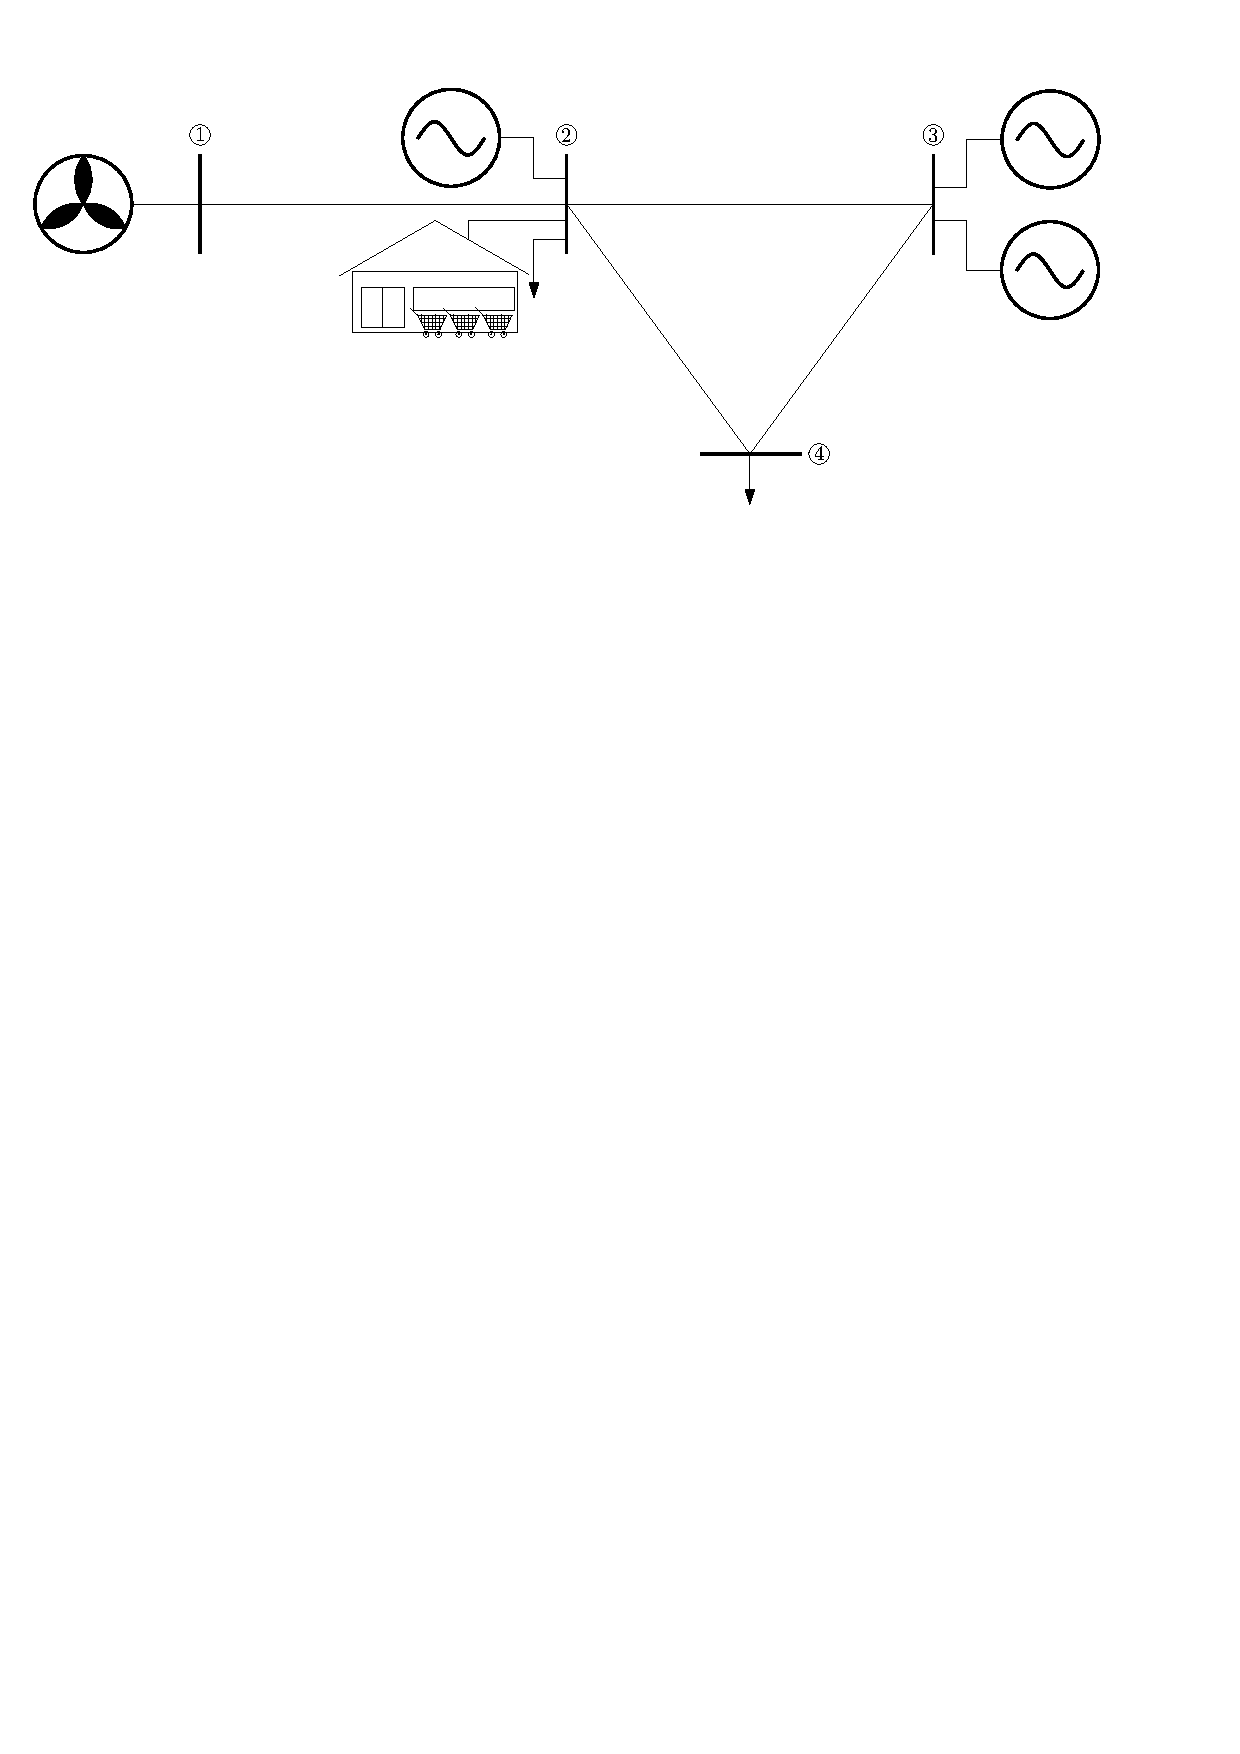
\includegraphics[scale=0.75]{images/SEVN/power_grid}
	\end{center}
\end{figure}

In der Realität kann ein Energieversorgungsnetz durch die Variation der
Knotenzahl und die Vermaschung beliebig komplizierte Form aufweisen. Bei der
Umsetzung der gegebenen Situation im Programm.

\begin{figure}[h]
\caption{Klassendiagramm Modellkonstrukt}
	\label{klassendiagramm}
	\begin{center}
	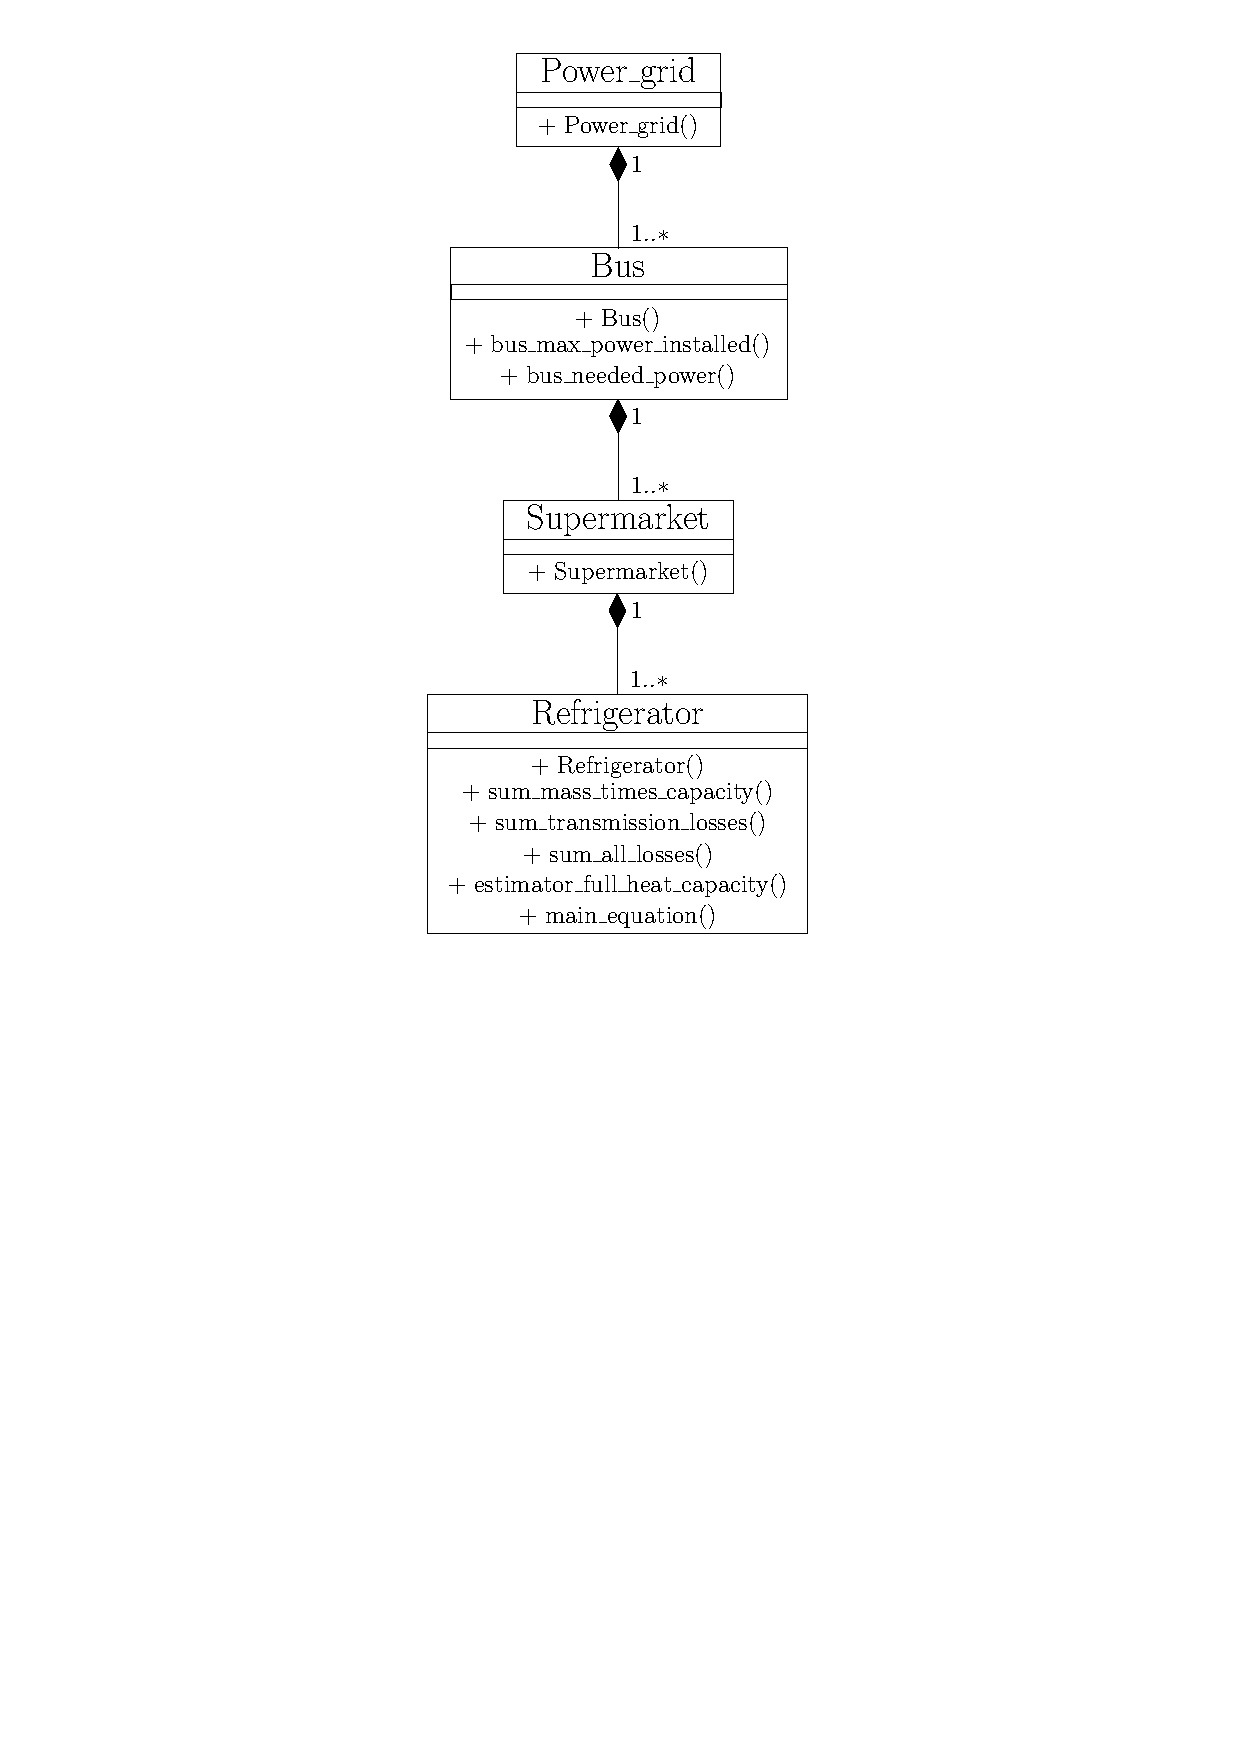
\includegraphics[scale=0.8]{images/Theorie_Super/class_diagramm}
	\end{center}
\end{figure}

Hier noch ein Zwischentext.

\begin{figure}[h]
\caption{Sequenzdiagramm Modellkonstrukt}
	\label{uml_sequence}
	\begin{center}
	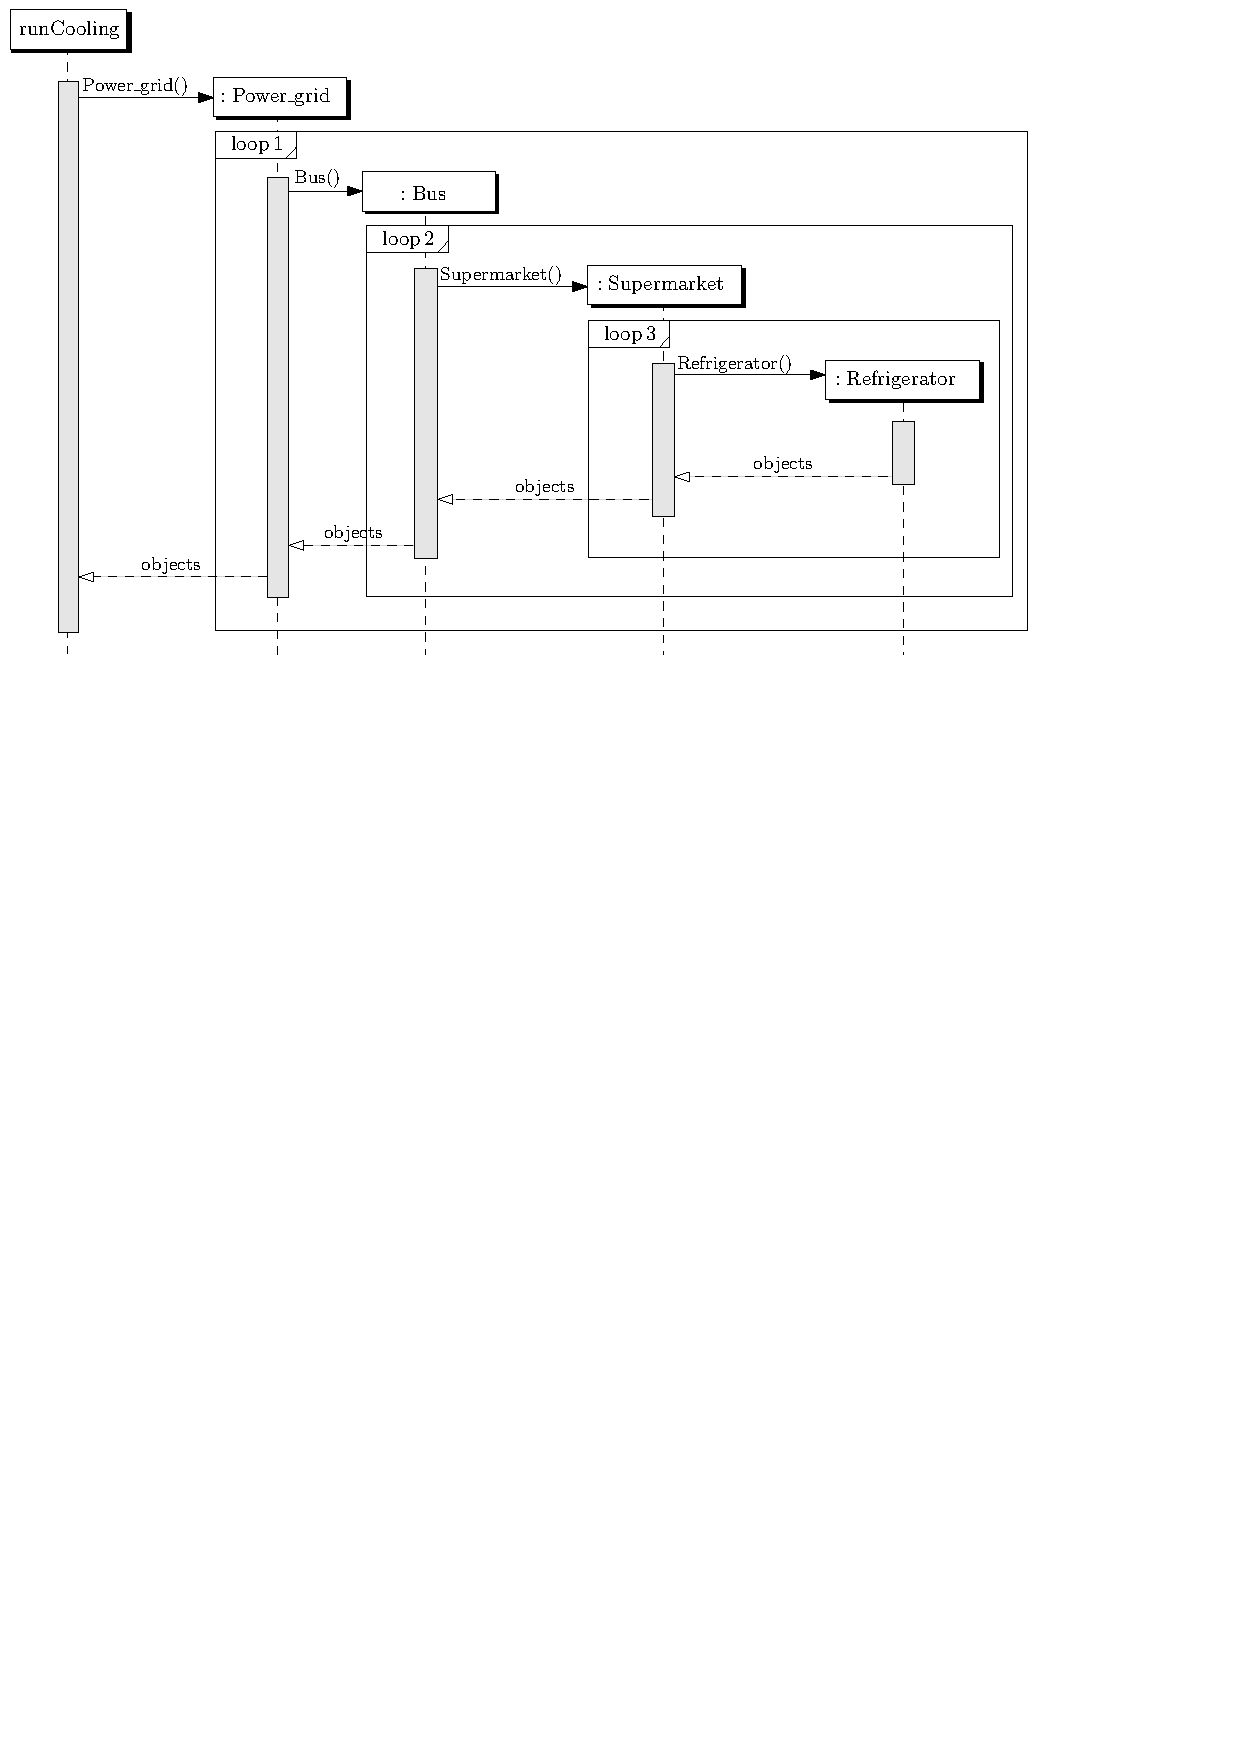
\includegraphics[scale=0.8]{images/Theorie_Super/sequence_one}
	\end{center}
\end{figure}

%%%%%%%%%%%%%%%%%%%%%%%%%%%%%%%%%%%%%%%%%%%%%%%%%%%%%%%%%%%%%%%%%%%%%%%%%%%%%%%%
%%%%%%%%%%%%%%%%%%%%%%%%%%%%%%%%%%%%%%%%%%%%%%%%%%%%%%%%%%%%%%%%%%%%%%%%%%%%%%%%

\section{Überblick über die mathematische Zusammenhänge}

In diesem Kapitel wird ein knapper \"Uberblick über die mathematischen und
physikalischen Zusammenhänge, die bei der Entwicklung eines Modellsupermarktes
zwingend beachtet werden müssen, vorgestellt\todo{Der Satz ist total scheiße
man}.

Die primäre Aufgabe der Kühleinheiten in einem Supermarkt besteht in der Regel
darin, Lebensmitteltemperatur unter die Zimmertemperatur zu bringen und diese
dabei zu halten\todo{Hört sich komisch an!}. Körper mit unterschiedlicher
Temperatur sind bestrebt, wenn sie thermisch von einander nicht vollkommen
isoliert sind, durch gegenseitige Wechselwirkung ihre Temperaturen anzugleichen,
sodass ein Wärmegleichgewicht entsteht, wobei der natürliche, selbständige
Wärmefluss immer von einem Körper mit höheren Temperatur in Richtung des Körpers
mit kleineren Temperatur stattfindet. Um eine negative Temperaturänderung
herzustellen und diese auch zu halten, muss die eindringende Wärmeenergie
ständig in der selben Höhe abgeführt werden, damit die Temperatur konstant
bleibt. Diese Energiemenge pro Zeiteinheit wird als Kälteleistung bezeichnet.
Eine Abweichung von dieser Menge führt zum Steigen der Temperatur, wenn weniger
und zum sinken der Temperatur wenn mehr abgeführt wird. Um diesen Kühlkreislauf
aufrecht zu erhalten, muss Leistung aufgewendet werden\footnote{ Eine
detailierte Beschreibung dieser Prozesse in einer Kopressionskälteanlage und
Spezifikation ist nicht Gegenstand dieser Arbeit.  Ausführliche Informationen
dazu findet man z.B.  in \cite{caro, doctor, TAB_A1}.}.

Das wird ausformuliert und mit einem Bild visualisiert\todo{bald schnell
machen}.
\begin{itemize}
	\item Temperaturunterschied in Kelvin $K$
	\item Wärmeausgleich (Verlust an Kälte)
	\item Kälteenergie gespeichert in Körpern mit einer bestimmten
	spezifischen Wärmekapazität
	\item Kälteenergie gespeichert in Masse
\end{itemize}
\begin{figure}\caption{ Modellgrundlage}
	\missingfigure{Modellgrundlage}
\end{figure}

Aufnahme der Wärmeenergie und der spezifischen Wärmekapazität dieser
Substanzmasse ergibt die Temperaturdifferenz $\Delta\:t$.

\begin{equation}
	\Delta\:t = \frac{Q}{m\cdot c}
\label{tdif}
\end{equation}

\begin{description}[\dth]

	\item[$\Delta\:t$] Temperaturdifferenz in Kelvin $K$
	\item[$Q$] Eindringende Wärmeenergie in $kJ$
	\item[$m$] Substanzmasse zur Aufnahme der Wärmeenergie in $kg$
	\item[$c$] Spezifische Wärmekapazität der Substanzmasse in $\frac{kJ}{kg
		\cdot K}$

\end{description}
\vspace{0.5cm}

Die installierte Kälteleistung multipliziert mit der täglichen Betriebszeit muss
zwangsweise größer oder gleich dem stündlichen Kältebedarf multipliziert mit der
Tagesstundenzahl sein.

\begin{equation}
	\pinstall = \frac{24\,h}{ \tau_{B} }  \cdot \pkalt \label{pinstall}
\end{equation}

\begin{description}[\dth]

	\item[$\pinstall$] Installierte Kälteleistung in $kW$
	\item[$\tau_{B}$] Tägliche Betriebszeit in $h$
	\item[$\pkalt$] Kältebedarf in $kW$

\end{description}
\vspace{0.5cm}

Die Transmissionswärmeleistung wird aus der Multiplikation der Fläche
der wärmeübertragenden Wänd mit ihrem spezifischen Wärmedurchgangskoeffizient
und der Temperaturdifferenz zwischen der Kühlraumtemperatur und der
Umgebungstemperatur berechnet.

\begin{equation}
	\ptrans = A \cdot k \cdot \Delta t
	\label{ptrans}
\end{equation}

\begin{description}[\dth]

	\item[$\ptrans$] Transmissionswärmeleistung in $kW$
	\item[$A$] Fläche in $m^2$
	\item[$k$] Wärmedurchgangskoeffiziente in $\frac{W}{m^2 \cdot K}$
	\item[$\Delta\: t$] Temperaturdifferenz in $K$

\end{description}
\vspace{0.5cm}

Der Zusammenhang zwischen der aufgewendeten elektrischen Antriebsleistung $P$
eines Verdichters in einer Kompressionskälteanlage und der genutzten
Kälteleistung ${\dot{Q}}_0$ wird durch die Kältezahl $\epsilon$ wiedergegeben.
Die Leistungszahl wird in die zweite Spalte im Array (vergl. Zeile 4 im
\matref{fridge}) eingetragen.

\begin{equation}
	\epsilon = \frac{\pkalt}{P}
\label{epsilon}
\end{equation}

\begin{description}[\dth]

	\item[$\epsilon$] Leistungszahl (einheitenlos)
	\item[$\pkalt$] Kälteleistungsbedarf in $kW$
	\item[$P$] elektrische Verdichterantriebsleistung in einer
		Kopressionskälteanlage in $kW$

\end{description}
\vspace{0.5cm}

Die Öffnungszeit des Supermarkts hat einen spürbaren Einfluss auf die Größe der
Wärmeverluste. In der Literatur wird der Nachtverbrauch mit $10\%$ bis $20\%$
des Tagesverbrauchs angegeben\cite{kauffeld}.  In der Nacht fallen keine
zusätzlichen Verluste zum Beispiel durch Licht, Körperwärme oder
Türöffnungszeiten, sodass nur Transmissionsverluste bei der Berechnung beachtet
werden.

\begin{equation}
	\dot{Q}_{Nacht}=\ptrans
\label{pnacht}
\end{equation}

\begin{description}[\dth]

	\item[$\pnacht$] Leistungsbedarf in der Nacht in $kW$
	\item[$\ptrans$] Transmissionswärmeleistung in $kW$

\end{description}
\vspace{0.5cm}


Der Leistungsbedarf am Tag ergibt sich aus der Summe des Tagesmehrbedarfs und
der Transmissionswärmeleistung. Aus Gründen der Vereinfachung wird
Tagesmehrbedarf als weitgehend konstant angenommen.

\begin{equation}
	\ptag = \pmehr + \ptrans
\label{ptag}
\end{equation}

\begin{description}[\dth]

	\item[$\ptag$] Leistungsbedarf am Tag in $kW$
	\item[$\pmehr$] Mehrbedarf am Tag in $kW$
	\item[$\ptrans$] Transmissionswärmeleistung in $kW$

\end{description}
\vspace{0.5cm}

Die Berechnung der mittleren Transmissionswärmeleistung erfolgt durch die
Multiplikation der Differenz zwischen der Umgebungstemperatur und der mittleren
Kühlraumtemperatur mit dem Wärmedurchgangskoeffizienten und der Fläche der
wärmeübertragenden Wände.

\begin{equation}
	\aptrans = A \cdot k \cdot \left( t_{amb} -
	\overline{t}_{KR} \right) \label{aptrans}
\end{equation}

\begin{description}[\dth]

	\item[$\aptrans$] mittlere Transmissionswärmeleistung in $kW$
	\item[$A$] Fläche in $m^2$
	\item[$k$] Wärmedurchgangskoeffiziente in $\frac{W}{m^2 \cdot K}$
	\item[$t_{amb}$] Umbgebungstemperatur in $^{\circ}C$
	\item[$\overline{t}_{KR}$] mittlere Kühlraumtemperatur in
		$^{\circ}C$
\end{description}
\vspace{0.5cm}

Ist f\"ur eine K\"alteanlage der K\"alteleistungsbedarf bekannt so wird der
Tagesmehrbedarf an K\"alteleistung ermittelt, indem vom Produkt des
K\"alteleistungsbarfes f\"ur $24\;h$ mit dem Faktor f\"ur
K\"altebedarfsabsenkung die mittlere Transmissionswärmeleistung abgezogen wird.

\begin{equation}
	\pmehr = \pkalt \cdot K - \aptrans
\label{pmehr}
\end{equation}

\begin{description}[\dth]

	\item[$\pmehr$] Mehrbedarf am Tag in $kW$
	\item[$\pkalt$] Kälteleistungsbedarf in $kW$
	\item[$K$] Faktor für Kältebedarfsabsenkung (einheitenlos)
	\item[$\aptrans$] mittlere Transmissionswärmeleistung in $kW$

\end{description}
\vspace{0.5cm}

Ist der Kälteleistungsbedarf nicht bekannt, wie zum Beispiel bei steckerfertigen
Geräten, kann der Mehrbedarf am Tag \"uber den Wert Verdichterarbeit pro 24
Stunden $\lverd$ für den gesamten Kälteverbraucher ermittelt werden.

Das Produkt aus dem spezifischen Energieverbrauch mit dem Faktor für
Kältebedarfsabsenkung, dem Verdichteranteil und der Anzahl der Geräte ergibt die
Verdichterarbeit.

\begin{equation}
	\lverd = \lspez \cdot K \cdot v \cdot n
\label{lverd}
\end{equation}

\begin{description}[\dth]

	\item[$\lverd$] Verdichterarbeit pro $24\,h$ in $\frac{kWh}{24h}$
	\item[$\lspez$] spezifischer Energieverbrauch pro $24\,h$ in
		$\frac{kWh}{24h}$
	\item[$K$] Faktor für Kältebedarfsabsenkung (einheitenlos)
	\item[$v$] Verdichteranteil (einheitenlos)
	\item[$n$] Anzahl der Geräte

\end{description}
\vspace{0.5cm}

Im Folgenden muss die Verdichterarbeit zum Abf\"uhren von zus\"atzlich
eindringenden W\"aremeenergie in der \"Offnungszeit berechnet werden, die einem
weiteren Schritt in W\"armeleistung $\pmehr$ umgewandelt wird.

\begin{equation}
	\lmehr = \lverd - \frac{\ptrans}{\epsilon} \cdot 24h
\label{lmehr}
\end{equation}

\begin{description}[\dth]

	\item[$\lmehr$] Verdichterarbeit zum Abführen von eindringenden
		Wärmeenergie $\emehr$ in $kWh$ in der \"Offnungszeit
	\item[$\lverd$] Verdichterarbeit pro $24\,h$ in $\frac{kWh}{24h}$
	\item[$\ptrans$] Transmissionswärmeleistung in $kW$
	\item[$\epsilon$] Leistungszahl (einheitenlos)

\end{description}
\vspace{0.5cm}

Die Umrechnung von $\lmehr$ in $\pmehr$ erfolgt mit Hilfe der Leistungszahl
$\epsilon$. Die Verdichterarbeit $\lmehr$ wird mit $\epsilon$ multipliziert.
Es wird angenommen, dass der Mehrbedarf in den rund zw\"olf Stunden der
\"Offnungszeit einf\"a

\begin{equation}
	\pmehr = \frac{\lmehr}{12h} \cdot \epsilon
\label{<++>}
\end{equation}

\begin{description}[\dth]

	\item[$\pmehr$] Mehrbedarf am Tag in $kW$
	\item[$\lmehr$] Verdichterarbeit zum Abführen von eindringenden
		Wärmeenergie $\emehr$ in $kWh$ in der \"Offnungszeit
	\item[$\epsilon$] Leistungszahl (einheitenlos)

\end{description}
\vspace{0.5cm}
berechnen.

Dabei entspricht $\pnacht$ der mittleren Transmissionswärmeleistung $\ptrans$.
$\ptag$ ist der Kältebedarf $\pkalt$, multipliziert mit dem Faktor für die
Kältebedarfsabsenkung $K$ bei Geräten, bei denen der Kältebedarf gegeben ist.
Bei steckerfertigen Geräten ist $\ptag$ die Summe aus dem Mehrbedarf an Leistung
am Tag $\pmehr$ und der mittleren Transmissionswärmeleistung $\ptrans$.

Mit den Wärmeverlusten, die am Tag und in der Nacht in unterschiedlicher Größe
auftreten, wird für jeden Zeitschritt die Zeit bis zum kritischen
Temperaturmaximum bestimmt. Diese Zeit braucht das Programm, um den Einsatz der
Supermarktkälteanlagen als Speicher zu planen. Mit der Gleichung

\begin{equation}
	\tau_{krit}(i) = \frac{m \cdot c \cdot (t_{max} -
		t(i))}{\aptranslog}
\label{taukn}
\end{equation}

\begin{description}[\dth]

	\item[$\tau_{krit}$] Zeit bis zur kritischen Temperatur in $h$
	\item[$m$] Substanzmasse zur Aufnahme der Wärmeenergie in $kg$
	\item[$c$] Spezifische Wärmekapazität der Substanzmasse in $\frac{kJ}{kg
		\cdot K}$
	\item[$t_{max}$] obere Temperaturgrenze in $ ^{\circ} C $
	\item[$t(i)$] Temperatur zur Stunde $i$ in $ ^{\circ} C $
	\item[$\aptranslog$] logrithmierte Mittelwert der
		Transmissionswärmeleistung in $kW$|
\end{description}
\vspace{0.5cm}


wird die Zeit $\tau_{krit}$ für jeden Zeitpunkt $i$ berechnet, wobei
$\overline{\dot{Q}}_{Tr_{ln}}$ der logarithmische Mittelwert ist, der sich aus
den Transmissionswärmeleistungen zum jeweils aktuellen Zeitpunkt $i$ mit der
Temperatur $t(i)$ und den Transmissionswärmeleistungen zum Zeitpunkt, an dem der
Kühlinnenraum die maximale Temperatur $t_{max}$ erreicht hätte, berechnet. Am
Tag müssen die restlichen Verluste $\pmehr$ zusätzlich zu den
Transmissionwärmeverlusten für die Berechnung der Zeit bis zur kritischen
Temperatur berücksichtigt werden, wodurch sich folgende Gleichung ergibt:

\begin{equation}
	\tau_{krit}(i) = \frac{m \cdot c \cdot (t_{max} -
		t(i))}{{\overline{\dot{Q}}_{Tr_{ln}}} + \pmehr}
\label{taukd}
\end{equation}

\begin{description}[\dth]

	\item[$\tau_{krit}$] Zeit bis zur kritischen Temperatur in $h$
	\item[$m$] Substanzmasse zur Aufnahme der Wärmeenergie in $kg$
	\item[$c$] Spezifische Wärmekapazität der Substanzmasse in $\frac{kJ}{kg
		\cdot K}$
	\item[$t_{max}$] obere Temperaturgrenze in $ ^{\circ} C $
	\item[$t(i)$] Temperatur zur Stunde $i$ in $ ^{\circ} C $
	\item[$\aptranslog$] logrithmierte Mittelwert der
		Transmissionswärmeleistung in $kW$
	\item[$\pmehr$] Mehrbedarf am Tag in $kW$

\end{description}
\vspace{0.5cm}

Die Zeit $\tau_{krit}$ ist abhängig vom Anstieg der Temperaturen und dieser
wiederum von den eindringenden Wärmelasten.

Um den Temperaturausgleich in den Lebensmitteln im Algorithmus zu
berücksichtigen, werden deshalb die zu- und abgeführten Wärmeenergiemengen bei
der Berechnung der Temperatur für jeden Zeitschritt stets mit dem Faktor 0,8
multipliziert.  Die Gleichung zur stündlichen Berechnung der aktuellen
Temperatur ist damit:

\begin{equation}
	t(i+1) = 0.8 \cdot \frac{Q_v - Q_{ab}}{m \cdot c} + t(i)
\label{tns}
\end{equation}

\begin{description}[\dth]

	\item[$t$] Temperatur in $^{\circ} C$
	\item[$Q_v$] eindringende Verlustwärmemenge in $kJ$
	\item[$Q_{ab}$] abführende Wärmemenge in $kJ$

\end{description}
\vspace{0.5cm}

wobei $Q_v$ die aktuell eindringende Wärmeenergie und $Q_ab$ die abgeführte
Wärmeenergie ist.

\chapter{Aufgabenstellung}
\label{chap:aufst}

%%%%%%%%%%%%%%%%%%%%%%%%%%%%%%%%%%%%%%%%%%%%%%%%%%%%%%%
%%%%%%%%%%%%%%%%%%%%%%%%%%%%%%%%%%%%%%%%%%%%%%%%%%%%%%%
%%%%%%%%%%%%%%%%%%%%%%%%%%%%%%%%%%%%%%%%%%%%%%%%%%%%%%%

Die Intention der Arbeit, ist der objektorientierte Entwurf eines
\matlab-Programms zur Simulation des variablen Lastverhaltens von Kältelasten
mit Kältespeichern im Energieversorgungsnetz. 

Es sollen ausschlie\ss lich K\"alteanlagen modelliert werden, die in den
Superm\"arkten zum Einsatz kommen. Das Ergebnis der Simulation soll der
Verbrauch einer variabel gef\"uhrten Supermarktkette auf der Basis der einzelnen
in den Superm\"arkten eingesetzten K\"alteanlagen sein.

Verbrauchswerte in einem Lastflussoptimierungsprogramm zu verwenden.

\section*{Explizite Anforderungen}

Folgende explizite Anforderungen sind an das Programm gestellt:

\begin{itemize}
	\item Die Speicherung der f\"ur das Beschreiben der Modelle
	erforderlichen Parameter findet in einer Konfigurationsdatei statt.
	\item Der elektrische Energieverbrauch wird auf Grund der
	Modellparameter der Kältelasten sowie des gefahrenen Einsatzes der
	Kältelasten berechnet.
	\item Die Topologie des elektrischen Netzwerkes werden ber\"ucksichtigt.
	\item Die M\"oglichkeit einer eindeutigen Zuweisung der Verbrauchswerte
	f\"ur folgende Verursacher wird realisiert:
	\begin{itemize}
		\item Daten f\"ur jede K\"alteanlage werden einzeln gespeichert,
		wenn der Verbrauch mehrerer Anlagen simuliert wird.
		\item Daten f\"ur jede Supermarktkette werden einzeln
		gespeichert, wenn der Verbrach mehrerer Supermarktketten
		simuliert wird.
		\item Erfolgt die Simulation des Energieverbrauchs f\"ur ein
		Mehrknotennetz, so werden die Daten f\"ur jeden Knoten, einzeln
		gespeichert.
	\end{itemize}
\end{itemize}



\chapter{Modellierung}
\label{chap:SEVN}
\minitoc

Der durchschnittliche Energieverbrauch der Kälteanlagen je Supermaktkette
kann aufgrund der technischen Ausführung unterschiedlich sein. Der
Energieverbrauch entsteht an definierten Punkten im Netz. An den einzelnen
Knotenpunkten können mehrere Kältelasten angeschlossen sein.

%%%%%%%%%%%%%%%%%%%%%%%%%%%%%%%%%%%%%%%%%%%%%%%%%%%%%%%%%%%%%%%%%%%%%%%%%%%%%%%%
%%%%%%%%%%%%%%%%%%%%%%%%%%%%%%%%%%%%%%%%%%%%%%%%%%%%%%%%%%%%%%%%%%%%%%%%%%%%%%%%

\section{Erstellung des OOP-Modells}

In der \cref{fig:vkb} wird ein einfaches Energieversorgungsnetz mit vier Knoten
dargestellt. Am Knoten eins ist eine regenerative elektrische Energiequelle, in
diesem Fall ein Windpark, angeschlossen. Weitere konventionelle elektrische
Energiequellen befinden sich an den Knoten zwei und drei. Die passiven Lasten
befinden sich am Knoten zwei und vier. Der Kältespeicher ist am Knoten zwei
angeschlossen. Im Bild wird der Kältespeicher Supermarkt durch ein Geb\"aude
mit Einkaufswagen dargestellt. Die Knoten sind untereinander durch Leitungen
verbunden.

\begin{figure}[h]
	\begin{center}
	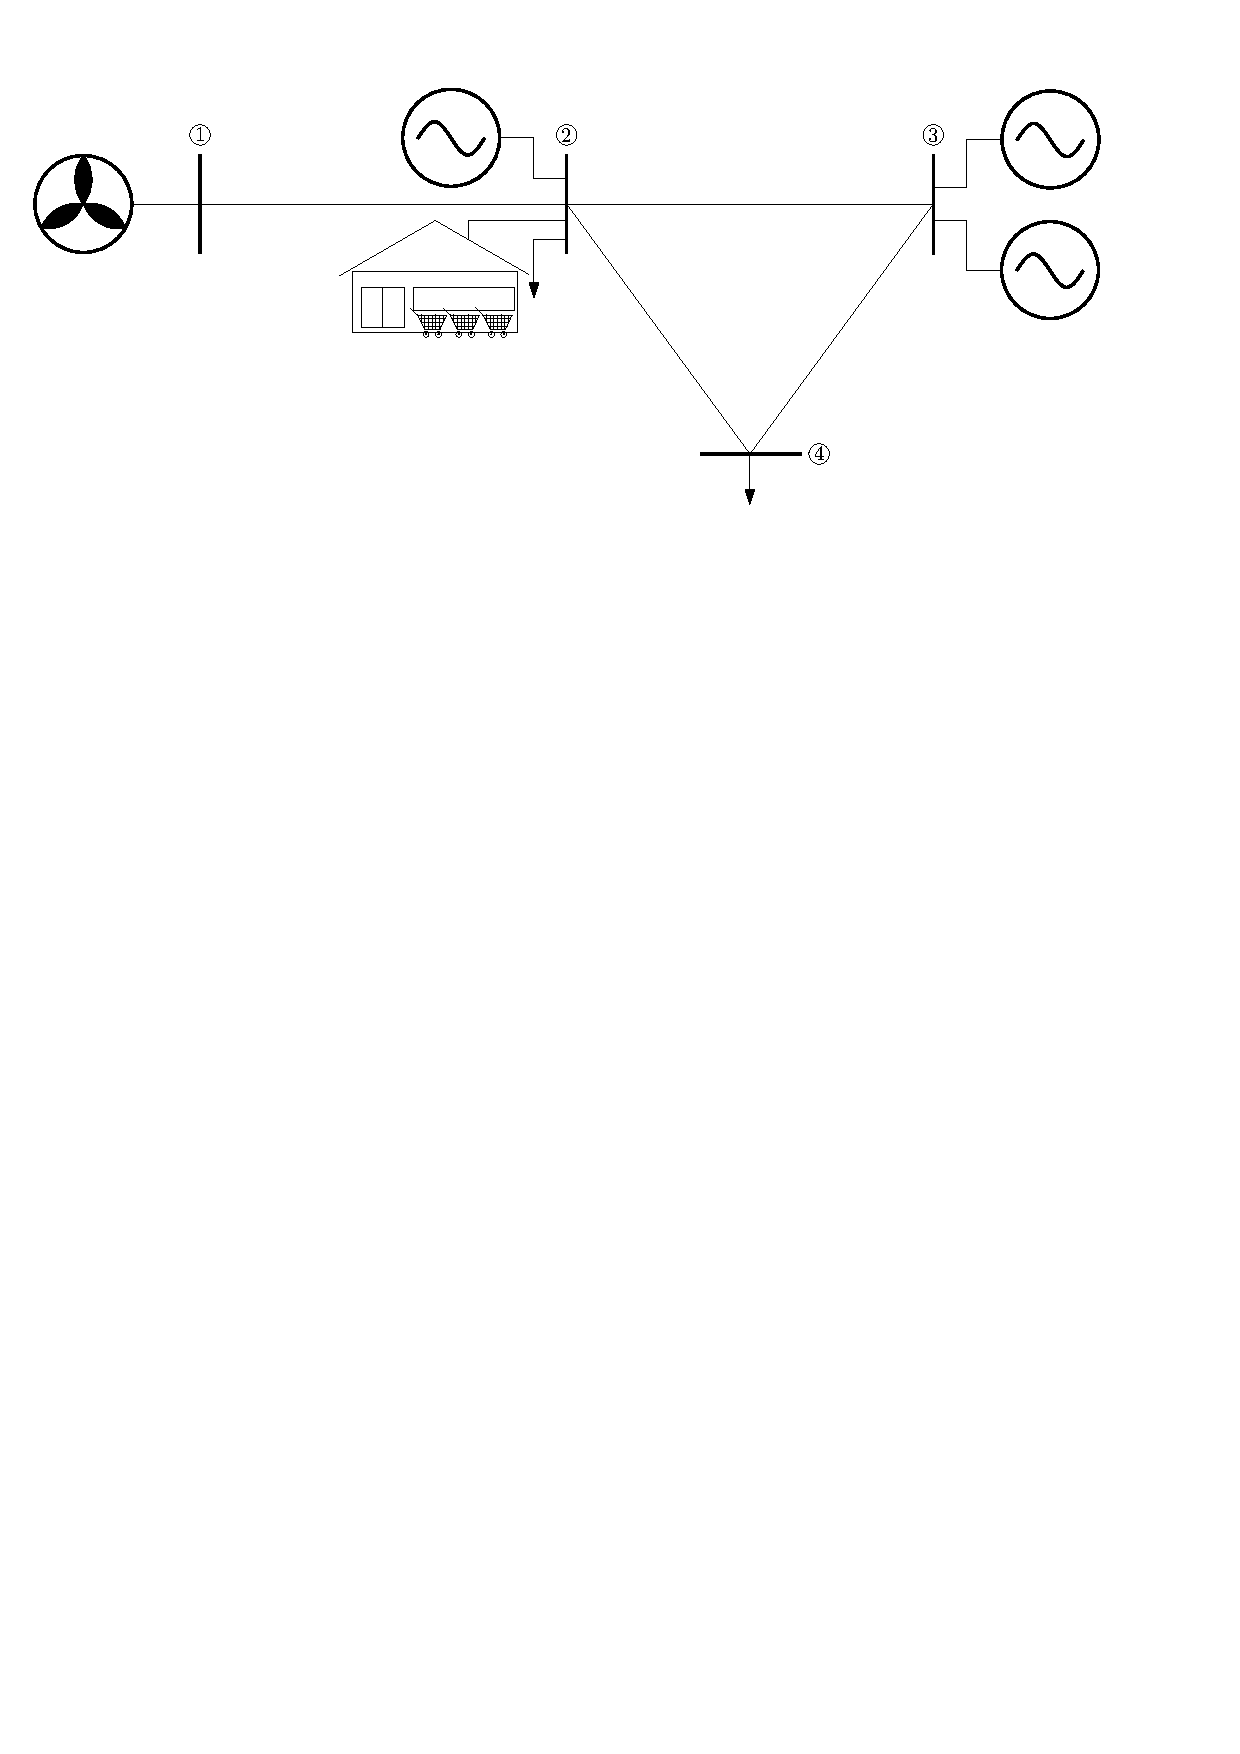
\includegraphics[scale=0.75]{images/SEVN/power_grid}
	\end{center}
\caption{Vier Knoten Beispiel}
\label{fig:vkb}
\end{figure}

\noindent In der Realität kann ein Energieversorgungsnetz durch die Variation
der Knotenzahl und die Vermaschung beliebig komplizierte Form aufweisen. \\

In Anbetracht der im \cref{sec:OOP} vorgestellten Verfahren erscheint der Ansatz
der OOP bei der Erstellung eines Programms zur Simulation einer K\"alteslast mit
K\"altespeicher im Energieversorgungsnetz auf der Basis des vorangegangenen
Beispiels (\cref{fig:vkb} auf der Seite \pageref{fig:vkb}) als sinnvoll. In der
\cref{fig:klassendiagramm} auf der Seite \pageref{fig:klassendiagramm} wird in
Form eines Klassendiagramms das fertige Klassen-Modell dargestellt und die
Abh\"angigkeit unter Klassen visualisiert.

\begin{figure}[h!]
	\begin{center}
	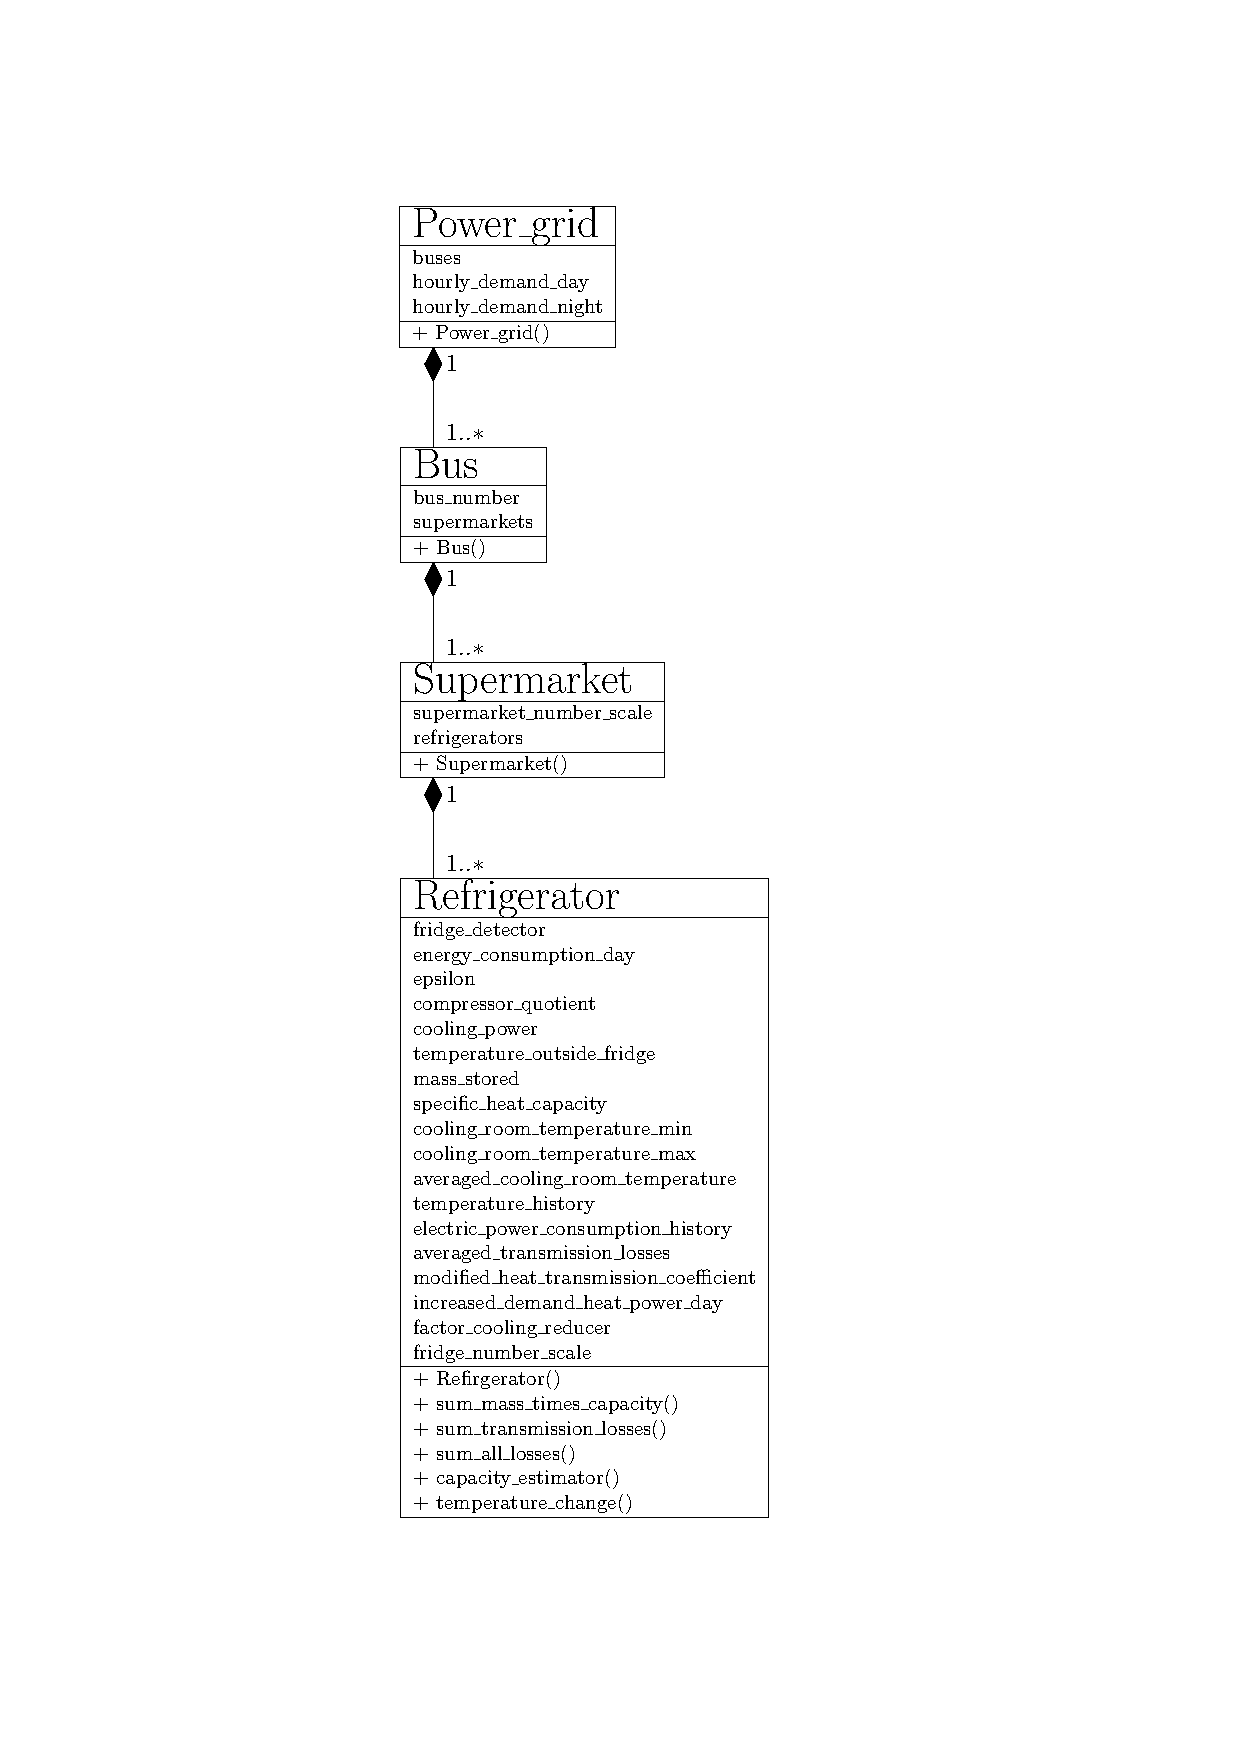
\includegraphics[scale=0.7]{images/Theorie_Super/class_new_diagramm}
	\end{center}
\caption{Klassendiagramm Modellkonstrukt}
\label{fig:klassendiagramm}
\end{figure}

Das Ergebnis der Abstraktion sind vier Klassen. In der Klasse
\textbf{Refrigerator} sind Eigenschaften und Methoden zusammengefasst, die das
Modell einer K\"altelast beschreiben. Die explizite Erkl\"arung der\todo{hier
ein \"Uberleitungssatz}.

\subsection*{Refrigerator}

An dieser Stelle werden die Eigenschaften und die Methoden der Klasse
\textbf{Refrigerator} explizit erkl\"art.

\subsubsection*{Attribute}
\begin{description}
	\item[fridge\_detector] Art der Anlage. Die Berechnung der Verluste der
	Verbundsanlagen unterscheidet sich von der der steckerfertigen
	Ger\"aten.
	\item[energy\_consumption\_day] H\"ohe des durchschnittlichen
	elektrischen Energieverbrauches.
	\item[epsilon] Leistungszahl.
	\item[compressor\_quotient] Anteil des Verdichters am Gesamtverbrauch
	der K\"uhlanlage.
	\item[cooling\_power] K\"alteleistungsbedarf (Herstellerangaben).
	\item[temperatur\_outside\_fridge] $1\times M$-Array mit
	Au\ss entemperaturwertet f\"ur die Umgebung der K\"alteanlage. $M$
	stimmt mit der Anzahl der W\"ande \"uberein, f\"ur die ihre Fl\"ache
	bekannt ist.
	\item[mass\_stored] $1\times N$-Array mit den Massewerten, der zur
	K\"uhlung vorhandenen Substansmasse. $N$ stimmt mit der Anzahl der
	Massen \"uberein, f\"ur die die spezifische W\"armekapazit\"at
	unterschiedlich ist.
	\item[specific\_heat\_capacity] $1\times N$-Array mit den Werten f\"ur
	spezifische W\"armekapazit\"aten der Substanzmassen.
	\item[cooling\_room\_temperature\_min] Niedrigste Temperatur, die durch
	K\"uhlung erreicht werden darf.
	\item[cooling\_room\_temperature\_max] H\"ochste Temperatur, die durch
	K\"uhlung erreicht werden darf.
	\item[averaged\_cooling\_room\_temperature] Durchschnittliche Temperatur
	im Normalbetrieb.
	\item[temperature\_history] $n \times m$-Array mit $(n,m)\in
	\mathbb{Z}^+_0$, wobei $n$ f\"ur die Anzahl der Werten des berechneten
	Temperaturverlaufes und $m$ f\"ur die Anzahl der simulierten Tage
	stehen\todo{stehen oder steht?}. Die Werte sind das Ergebnis der
	Berechnung der Funktion \textbf{main\_equation}. Eine Spalte des Arrays
	stellt den Temperaturverlauf an genau einem Tag dar.
	\item[electric\_power\_consumption\_history] $n \times m$-Array mit
	$(n,m)\in \mathbb{Z}^+_0$, wobei $n$ f\"ur die Anzahl der Werten des
	berechneten Verbrauchs und $m$ f\"ur die Anzahl der simulierten Tage
	stehen\todo{stehen oder steht?}. Die Werte sind das Ergebnis der
	Berechnung der Funktion \textbf{main\_equation}. Eine Spalte des Arrays
	stellt den Verlauf des berechneten Verbrauches an genau einem Tag dar.
	\item[averaged\_transmission\_losses] Summe aller durchschnittlichen
	Transmissionsverluste im Normalbetrieb (vgl. \cref{aptrans} auf der
	Seite \pageref{aptrans}).
	\item[modified\_heat\_transmission\_coefficient] $1\times M$-Array mit
	Werten aus der elementenweise Multiplikation des Vektors mit Werten der
	spezifischen W\"armedurchgangskoeffizienten mit dem Vektor mit Werten
	f\"ur die Durchgagnsfl\"achen (vgl. \cref{vmod} auf der Seite
	\pageref{vmod}).
	\item[increased\_demand\_heat\_power\_day] Mehrbedarf am Tag, aufgrund
	der zus\"atzlichen Verluste durch Licht, Menschenk\"orperw\"arme,
	T\"ur\"offnungszeiten und weiteren Einfl\"usse. Die Berechnung erfolgt
	nach einer Auswahl zwischen der \cref{pmehr} und der \cref{lverd} bis
	\cref{spmehr} wie auf der Seiten \pageref{pmehr} und \pageref{spmehr}
	beschrieben.
	\item[factor\_cooling\_reducer] Faktor f\"ur K\"altebedarfsabsenkung
	infolge der Luftfeuchtigkeit und der Umgebungstemperatur.
	\item[fridge\_number\_scale] Anzahl der Anlagen mit der identischen
	technischen Ausf\"uhrung, der Beladung und dem Fahrplan.
\end{description}

\subsubsection*{Methoden}
\begin{description}
	\item[Refrigerator(fridge\_config,number\_steps,days)] Konstruktor der
	Klasse. Bei dem Aufruf dieser Funktion werden folgende Argumente
	\"ubergeben:
	\begin{description}
		\item[fridge\_config] $1 \times 2$-Cell Array
		mit Modellparametern\footnote{ Die Form des Arrays ist
		\"aquivalent zu genaue einer Zeile der in
		\matref{csuper} auf der Seite \pageref{csuper} vorgestellten
		Arrays, die die Modelle der Superm\"arkte abbilden.}.
		\item[number\_steps] Anzahl der Zeitschritte die einen
		Tag beschreiben.
		\item[days] Anzahl der zu simulierenden Tage.
	\end{description}
	Bei der Initialisierung eines Objektes werden einem Teil der oben
	vorgestellten Attribute der Klasse \textbf{Refrigerator} Werte aus dem
	\textbf{ fridge\_config }-Array direkt \"ubergeben. Andere Werte werden
	einmalig von der Konstruktor-Methode berechnet oder im Laufe der
	Simulation ver\"andert.\\

	Folgende Attribute werden einmalig bei der Initialisierung berechnet:
	\begin{description}
		\item[averaged\_transmission\_losses] Summe aller
		durchschnittlichen Transmissionsverluste im Normalbetrieb
		(vgl. \cref{aptrans} auf der Seite \pageref{aptrans}).
		\item[modified\_heat\_transmission\_coefficient] $1\times
		M$-Array mit Werten aus der elementenweise Multiplikation des
		Vektors mit Werten der spezifischen
		W\"armedurchgangskoeffizienten mit dem Vektor mit Werten f\"ur
		die Durchgagnsfl\"achen (vgl. \cref{vmod} auf der Seite
		\pageref{vmod}).
		\item[increased\_demand\_heat\_power\_day] Mehrbedarf am Tag ,
		aufgrund der zus\"atzlichen Verluste durch Licht,
		Menschenk\"orperw\"arme, T\"ur\"offnungszeiten und weiteren
		Einfl\"usse. Die Berechnung erfolgt nach einer Auswahl
		zwischen der \cref{pmehr} und der \cref{lverd} bis \cref{spmehr}
		wie auf der Seiten \pageref{pmehr} und \pageref{spmehr}
		beschrieben.
	\end{description}

	Folgende Attribute werden im Laufe der Simulation ver\"andert:
	\begin{description}
		\item[temperature\_history] $n \times m$-Array mit $(n,m)\in
		\mathbb{Z}^+_0$, wobei $n$ f\"ur die Anzahl der Werten des
		berechneten Temperaturverlaufes und $m$ f\"ur die Anzahl der
		simulierten Tage stehen\todo{stehen oder steht?}. Die Werte sind
		das Ergebnis der Berechnung der Funktion
		\textbf{main\_equation}. Eine Spalte des Arrays stellt den
		Temperaturverlauf an genau einem Tag dar.
		\item[electric\_power\_consumption\_history] $n \times m$-Array
		mit $(n,m)\in \mathbb{Z}^+_0$, wobei $n$ f\"ur die Anzahl der
		Werten des berechneten Verbrauchs und $m$ f\"ur die
		Anzahl der simulierten Tage stehen\todo{stehen oder steht?}. Die
		Werte sind das Ergebnis der Berechnung der Funktion
		\textbf{main\_equation}. Die Werte sind das Ergebnis der
		Berechnung der Funktion \textbf{main\_equation}. Eine Spalte des
		Arrays stellt den Verlauf des berechneten Verbrauches an genau
		einem Tag dar.
	\end{description}

	Folgende Attribute sind auf Grund der Annahmen dieser Studie konstant,
	k\"onnen aber bei der bei einer Modifizierung der Annahmen im Laufe der
	Simulation ver\"andert werden:
	\begin{description}
		\item[temperature\_outside\_fridge] Befindet sich der
		K\"altespeicher au\ss erhalb geschlossener R\"aume und im
		direkten Kontakt mit der Au\ss entemperatur, muss die
		Temperatur\"anderung die im Tagesverlauf in Abh\"angigkeit von
		der Jahreszeit entsteht, beachtet werden.
		\item[mass\_stored] Wenn nicht mehr Angenommen wird, dass
		die Substansmasse im Supermarkt im Laufe des Tages konstant ist,
		sondern mit dem Konsumverhalten der Bev\"olkerung in
		Abh\"angigkeit steht, muss eine Anpassung erfolgen.
	\end{description}

	\item[sum\_mass\_times\_capacity()] Der R\"uckgabewert dieser Funktion
	ist die berechnete Summe aus elementenweise Multiplikation aller
	Substansmassen mit der jeweiligen spezifischen W\"armekapazit\"aten. Der
	Funktion werden keine explizite Argumente \"ubergeben. Die Funktion
	greift direkt auf die Attribute \textbf{specific\_heat\_capacity} und
	\textbf{mass\_stored} des Objektes zu\todo{Warum ist es n\"otig, die
	Funktion expliziert zu schreiben?}.

	\item[sum\_transmission\_losses()] Es gibt zwei R\"uckgabewerte dieser
	Funktion. Der erste Wert ist die Summe der Transmissionsverluste (vgl.
	\cref{aptrans} auf der Seite \pageref{ptrans}) durch alle
	Durchgangsfl\"achen f\"ur den aktuellen Zeitpunkt und die aktuelle
	K\"uhlraumtemperatur. Desweiteren wird die Summe der
	Transimissionsverluste berechnet, die bei der oberen Grenze des
	zugelassenen Temperaturbereiches entstehen. Die Kenntnis dieser Verluste
	ist wichtig um die Zeitspanne absch\"atzen zu k\"onnen, bis obere
	Temperaturgrenze erreicht wird (vgl. \cref{taukn} auf der Seite
	\pageref{taukn}).

	Die \"Ubergabe folgender Argumente an die Funktion ist erforderlich:
	\begin{description}
		\item[number\_steps] Laufvariable. Gesamtzahl der zu
		simulierenden Zeitschrite f\"ur ein Tag.
		\item[count\_number\_steps] Der aktuelle Wert von
		\textbf{number\_steps}.
		\item[count\_number\_day] Der aktuelle Wert von der Laufvariable
		\textbf{number\_days}.
	\end{description}

	\item[sum\_all\_losses()] Es gibt zwei R\"uckgabewerte dieser Funktion.
	Der erste R\"uckgabewert beinhaltet die Summe aller Verluste an K\"alte
	(vgl. \cref{qv} auf der Seite \pageref{qv}).
	Au\ss erhalb der \"Offnungszeiten entf\"allt der Anteil an
	zus\"atzlichen Verlusten, die durch Licht, offene T\"uren und etc.
	anfallen. Durch eine alternative Verzweigung, deren Bedingung die
	Zugeh\"origkeit des aktuellen Wertes der Laufvariable
	\textbf{count\_number\_steps} zu den \"Offnungszeiten ist, wird die
	Ber\"ucksichtigung der zus\"atzlichen Verluste sichergestellt. Der
	zweite Ruckgabewert ist die Zeitspanne bis zum Erreichen der kritischen
	maximalen Temperatur (vgl. \cref{taukn} und \cref{taukd} auf den Seiten
	\pageref{taukn} und \pageref{taukd}).

	Die \"Ubergabe folgender Argumente an die Funktion ist erforderlich:
	\begin{description}
		\item[number\_steps] Laufvariable. Gesamtzahl der zu
		simulierenden Zeitschrite f\"ur ein Tag.
		\item[count\_number\_steps] Der aktuelle Wert von
		\textbf{number\_steps}.
		\item[count\_number\_day] Der aktuelle Wert von der Laufvariable
		\textbf{number\_days}.
		\item[number\_days] Laufvariable. Gesamtzahl der zu
		simulierenden Tage.
	\end{description}

	\item[capacity\_estimator()] Die Funktion hat einen R\"uckgabewert.
	Berechnet wird die maximal abzuf\"uhrende Wermeenergiemenge $\emax$
	(vgl. die \cref{emax} auf der Seite \pageref{emax}).

	Die \"Ubergabe folgender Argumente an die Funktion ist erforderlich:
	\begin{description}
		\item[count\_number\_steps] Der aktuelle Wert von
		\textbf{number\_steps}.
		\item[count\_number\_day] Der aktuelle Wert von der Laufvariable
		\textbf{number\_days}.
		\item[Q\_losses] Wert der aktuellen eindringenden
		W\"armeenergie als Ergebnis der Funktion
		\textbf{sum\_all\_losses()}.
	\end{description}
	\item[temperature\_change()] Die Funktion hat einen R\"uckgabewert.
	Berechnet wird die Temperatur der Substanzmasse, die durch K\"uhlung am
	Ende eines Zeitschrittes erreicht wird (vgl. die \cref{tns} auf der
	Seite \pageref{tns}).
	
	Die \"Ubergabe folgender Argumente an die Funktion ist erforderlich:
	\begin{description}
		\item[number\_steps] Laufvariable. Gesamtzahl der zu
		simulierenden Zeitschrite f\"ur ein Tag.
		\item[count\_number\_steps] Der aktuelle Wert von
		\textbf{number\_steps}.
		\item[count\_number\_day] Der aktuelle Wert von der Laufvariable
		\textbf{number\_days}.
		\item[Q\_losses] Wert der aktuellen eindringenden
		W\"armeenergie als Ergebnis der Funktion
		\textbf{sum\_all\_losses()}.
	\end{description}
\end{description}

Alle Klassen haben einen unterschiedlichen Status. Die Klasse
\textbf{Power\_gird} vertritt die Rolle des ganzen Systems, also des
Energieversorgungsnetzes, welches aus charakteristischen Teilen, den Knoten
(\textbf{Bus}) besteht. Die Existenz eines Knotens au\ss erhalb eines Netzes
ergibt f\"ur die Berechnung keinen Sinn. Dieser Zusammenhang zwischen Klassen
wird im Klassendiagramm \cref{fig:klassendiagramm} durch eine Linienverbindung
verdeutlicht. Auf der Seite des Ganzen endet die Linie mit einem ausgef\"ullten
Rhombus. Das komplette Modell ist nach diesem Prinzip aufgestellt. Die kleinste
Einheit des Ganzen stellt die K\"alteanlage (\textbf{Refrigerator}) dar.

\begin{figure}[h]
	\begin{center}
		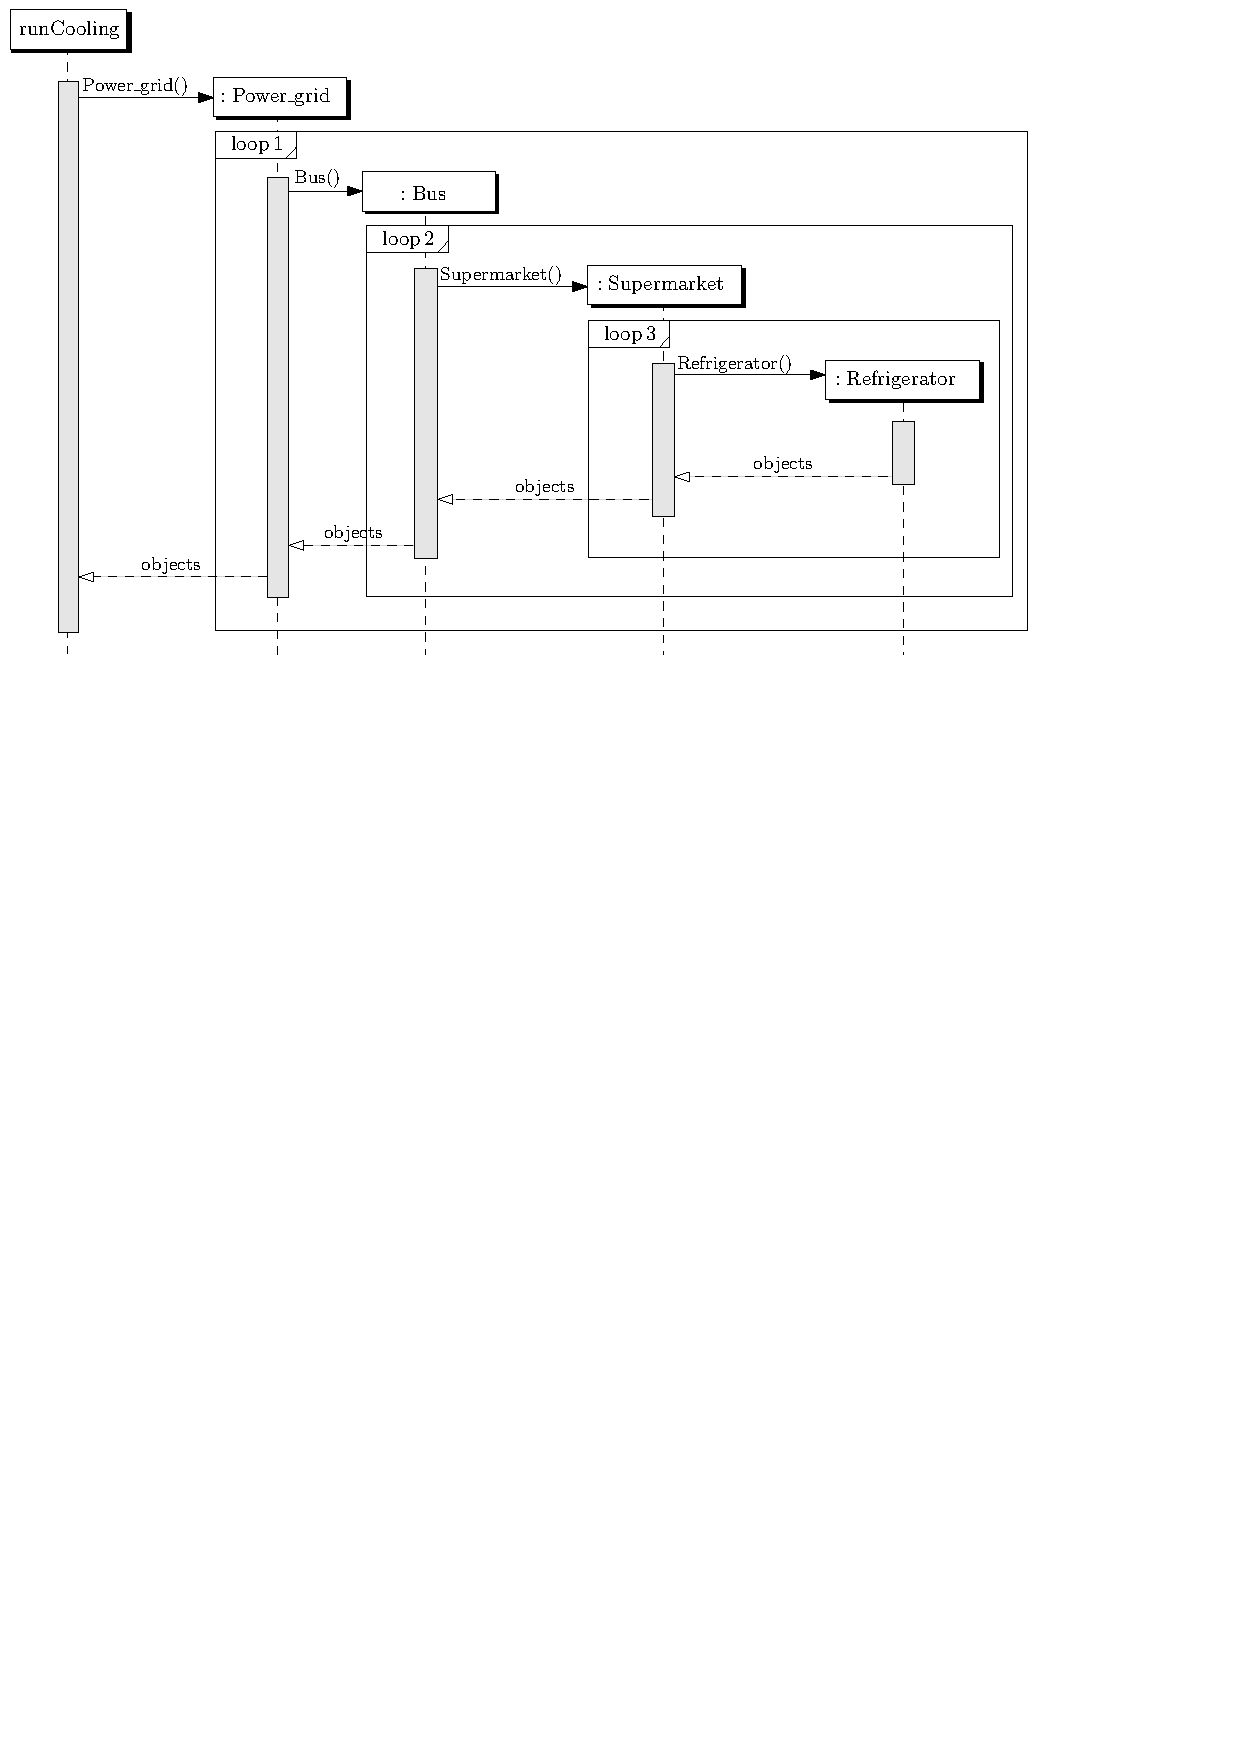
\includegraphics[scale=0.8]{images/Theorie_Super/sequence_one}
	\end{center}
\caption{Sequenzdiagramm Modellkonstrukt}
\label{fig:uml_sequence}
\end{figure}

Auf Grund des Modells wird das elektrische Verhalten einer
Supermarket-K\"altelast im Energieversorgungsnetz durch miteinander
kooperierende Objekte dargestellt. Wird eine Funktion aufgerufen, die den Start
der Simulation veranlasst, m\"ussen, bevor auf die Methoden der einzelnen
Objekte zugegriffen werden kann, die Objekte erzeugt werden.

In der \cref{fig:uml_sequence} auf der \pageref{fig:uml_sequence} wird mit Hilfe
eines Sequenzdiagrammes der Nachrichtenaustausch hervorgehoben, der bei der
Erstellung der Objekte durchlaufen wird. Auf der Zeitachse, die senkrecht von
oben nach unten verl\"auft, wird mit Hilfe der Pfeile der Zugriff auf die
Methoden der Objekte dargestellt. Ist eine Methode des Objektes f\"ur einen
Zeitraum aktiv, wird dieser Zustand durch einen grauen Balken auf dem Zeitstrahl
des zugeh\"origen Objektes visualisiert. Der Aufruf der Funktionen der Objekte
wird durch einen Pfeil mit ausgef\"ullter Spitze dargestellt. Der Pfeil geht vom
Zeitstrahl eines Objekts aus, der die Funktion aufruft und endet mit der Spitze
im Objekt, zu dem diese Funktion geh\"ort. Der Name der aufgerufenen Funktion
steht \"uber dem Pfeil. Wird von dieser Funktion etwas zur\"uckgegeben, so ist
der Pfeil gestrichelt. Ist Die R\"uckgabevariablen stehen \"uber dem Pfeil.

In der Funktion \textbf{runCooling}, die den Start der Simulation veranlasst und
steuert, wird der Konstruktor der Klasse \textbf{Power\_grid} aufgerufen. Als
Ergebnis des Aufrufes bekommt die Funktion \textbf{runCooling} ein Objekt der
Klasse \textbf{Power\_grid} mit allen Unterobjekten, die den zu simulierenden
Fall beschreiben. Die Konstruktor-Funktionen der Klassen, die einen
untergeordneten Status besitzen, werden bei der Erstellung der \"ubergeordneten
Objekte aufgerufen. Die Anzahl der erzeugten Objekte h\"angt davon ab, wie oft
die Konstruktor-Funktion der jeweiligen Klasse aufgerufen wird. Diese Zahlen
werden in Konfigurationsdateien abh\"angig von dem untersuchten Fall festgelegt.
Die ausf\"uhrliche Erkl\"arung der Konfigurationsdateien wird in kommenden
Abschnitten vorgenommen.

\subsection*{Bereitstellung der Leistung zur K\"alteerzeugung}

Der augenblickliche Gleichgewicht zwischen dem K\"altebedarf und der zur
Verf\"ugung stehenden K\"alteleistung sichert die Einhaltung der Soll-Temperatur
der K\"uhlg\"uter. Werden die K\"alteanlagen als Energiespeicher zur Regelung
eingesetzt, so f\"uhrt das auf Grund der fluktuierenden zur Verf\"ugung
stehenden K\"alteleistung zu Temperaturschwankungen. Die engen Grenzen des
zul\"assigen Temperaturbandes d\"urfen nicht \"uberschritten werden.

Verschiedene Konzepte f\"ur den Einsatz der K\"alteanlagen als Energiespeicher
im Energieversorgungsnetz sind denkbar. Im folgenden Abschnitt wird die
Implementierung eines m\"oglicher Kooperationskonzept zwischen Supermarkt und
Windpark vorgestellt.

Die prognostizierten elektrischen Windleistungsdaten und die tatsächlich vom
Windpark produzierten elektrischen Windleistungsdaten der Vattenfall-Regelzone
\todo{was ist das heute?} aus dem Jahr 2005 werden als Grundlage-Datensatz zur
Implementierung des Kooperationskonzeptes verwendet. Im Datensatz sind
Stundenwerte von Windleistung gespeichert weshalb in diesem Fall auch von
Energie gesprochen werden kann.

Der Windpark ist bestrebt die Verpflichtung \"uber die Bereitstellung von
Leistung beim Netzbetreiber zu erf\"uhlen. Abweichungen, die aufgrund der
fehlerhaften Windprognosen entstehen, sollen durch die Kooperation mit
Supermarktketten ausgeglichen werden.

Es wird angenommen, dass der Prognosefehler von der Windleistungsvorhersage
f\"ur 24 h den 15\% entspricht. Der Windparkbetreiber meldet beim Netzbetreiber
die untere Grenze, also 85\% von der Windleistungsvorhersage, an. Der
Supermarkt besitzt einen st\"undlichen Bedarf, der unbedingt gedeckt werden
muss. Sind die 15\% von der Prognose kleiner als der st\"undliche Bedarf, wird
die Differenz aus dem Netz gezogen. Diese Abweichung wird beim Netzbetreiber zur
Erstellung des Lastfahrplanes mitgeteilt. \"Ubersteigt der Prognosefehler die
15\%, versucht der Supermarkt diesen \"Uberschuss zu neutralisieren.

Die vom Windparkbetreiber beim Netzbetreiber anzumeldende Leistung wird
berechnet, indem von der Windleistungsvorhersage die 85\% bestimmt werden
oder der st\"undliche Bedarf des Supermarktes abgezogen wird, wenn die 15\%
kleiner als der st\"undliche Bedarf sind.
\begin{equation*}
	b = 0.85 \cdot P_{DA}
\end{equation*}
oder
\begin{equation*}
	b = P_{DA} - P_{dem}\\
	\label{b}
\end{equation*}

 \begin{description}[\dth]
	\item[$b$] Leistung, die vom Windparkbetreiber beim Netzbetreiber
	angemeldet wird in $MW$
	\item[$P_{DA}$] Vorhersage der Windleistung (day ahead) in $MW$
	\item[$P_{dem}$] st\"undlicher Leistungsbedarf des Supermarkts (demand)
	$MW$
 \end{description} \vspace{0.5cm}

Die vom Windparkbetreiber dem Supermarkt versprochene Leistung wird berechnet,
indem von der Windleistungsvorhersage die 15\% bestimmt werden oder nur der
st\"undliche Bedarf, wenn die 15\% kleiner als der st\"undliche Bedarf sind.
\begin{equation*}
	a = 0.15 \cdot P_{DA}\\
\end{equation*}
oder
\begin{equation*}
	a = P_{dem}\\
	\label{b}
\end{equation*}

\begin{description}[\dth]
	\item[$a$] Leistung, die vom Windparkbetreiber dem Supermarkt
	versprochen wird in $MW$
	\item[$P_{DA}$] Vorhersage der Windleistung (day ahead) in $MW$
	\item[$P_{dem}$] st\"undlicher Leistungsbedarf des Supermarkts (demand)
	$MW$
\end{description} \vspace{0.5cm}

Die Leistung, die insgesamt den K\"alteanlagen zur Verf\"ugung steht, berechnet
sich nach der \cref{pload}. Der Ausdruck $P_{RT} - b$ bedeutet die
\"ubersch\"ussige Windleistung. Der Ausdruck $P_{dem} - a$  bedeutet die vom
Supermarkts beim Netzbetreiber nicht abgemeldete Leistung.

\begin{equation}
	P_{load} = P_{RT} - b + P_{dem} - a
	\label{pload}
\end{equation}
\begin{description}[\dth]
	\item[$P_{load}$] vorhandene Leistung zum Laden in $MW$
	\item[$a$] Leistung, die vom Windparkbetreiber dem Supermarkt
	versprochen wird in $MW$
	\item[$P_{dem}$] st\"undlicher Leistungsbedarf des Supermarkts (demand)
	$MW$
\end{description} \vspace{0.5cm}

\subsubsection*{Implementierung}
Die Implementierung des Kooperationskonzeptes erfolgt in einer neuen Klasse
\textbf{Cooling\_strategy}. Diese Klasse hat die Aufgabe jeder K\"uhlstelle in
jedem Supermarkt im Netz die aufgrund des Kooperationskonzeptes und der
Temperaturbeschr\"ankungen optimale Menge an K\"alteleistung zuzuweisen. Die zur
Verf\"ugung vorhandene Leistung wird auf alle K\"uhlstellen gleichm\"a\ss ig
aufgeteilt bis keine Leistung mehr zur Verf\"ugung steht oder die
Minimaltemperatur erreicht wird. Alle K\"uhlstellen sollen zu jeder Stunde
mindestens soviel Leistung zugewiesen bekommen, dass genau diese eine Stunde
\"uberbr\"uckt werden kann, ohne dass die H\"ochsttemperatur \"uberschritten
wird.
\begin{figure}[h!]
	\begin{center}
	\includegraphics[scale=0.7]{images/Theorie_Super/class_diagramm_second}
	\end{center}
\caption{Klassendiagramm Kooperationskonzept}
\label{fig:klasskoop}
\end{figure}

In der \cref{fig:klasskoop} auf der Seite \pageref{fig:klasskoop} wird in einem
Klassendiagramm die Beziehung zwischen dem bestehenden Modell und der Klasse
\textbf{Cooling\_strategy} dargestellt. Eine Klasse \textbf{Cooling\_strategy}
steht in der direkten Verbindung mit der Klasse \textbf{Refrigerator}, f\"ur die
sie die zur K\"uhlung erforderliche Leistung berechnet. Ein Objekt der Klasse
\textbf{Cooling\_strategy} kann mit einem bis mehreren Objekten der Klasse
\textbf{Refrigerator} in Verbindung stehen.\\

In der \cref{fig:coop} auf der Seite \pageref{fig:coop} ist der
Programmstrukturplan der Kooperationskonzeptes dargestellt. Der Algorithmus
zeigt den Ablauf beim "'Auff\"uhlen"' der K\"uhlstellen in einer f\"ur genau
einen Zeitschritt der Simulation. Die Umsetzung des Algorithmus erfolgt in der
Funktion \textbf{strategy\_calculator()}.

\begin{description}
\item[strategy\_calculator()] Es gibt f\"unf R\"uckgabewerte dieser Funktion.
Der erste R\"uckgabewert ist ein $n\times11\,$-Array, wobei $n$ f\"ur die Anzahl
der im gesamten Netz vorhandenen K\"uhlzellen steht. In den Spalten des Arrays
werden alle Informationen gespeichert, die durch Berechnungen in der Funktion
entstanden sind und die Information zur eindeutigen Zuordnung dieser Ergebnisse
zu der jeweiligen K\"alteeinheit. ergibt sich dadurch, dass 
\end{description}

Der Auff\"uhlvorgang findet zwischen den st\"undlichen Temperaturberechnungen
statt. Diese Handlung wird schrittweise wiederholt, um das gleichm\"a\ss ige
Verteilung der Leistung auf alle Anlagen zu erm\"oglichnen. Zur L\"osung dieser
Aufgabe im Programm ist eine \textbf{while}-Schleife mit einer Abbruchbedingung
geeignet. Innerhalb der \textbf{while}-Schleife wird der Algorithmus
\cref{fig:coop} umgesetzt.

Im ersten Schritt des Algorithmus findet eine Abfrage statt, ob Leistung zum
K\"uhlen der Anlagen zur Verf\"ugung steht. Dieser Berechnung liegt die
Gleichung \cref{pload} auf der Seite \pageref{pload} zugrunde die in der
Funktion \textbf{power\_for\_load\_nett()} implementiert ist.
\begin{description}
\item[Fall 1] Die Menge der Leistung ist nicht gr\"o\ss er Null. Es erfolgt die
n\"achste Abfrage nach den K\"uhlstellen, die eine Stunde ohne Leistung aus dem
Netz nicht \"uberstehen k\"onnen, ohne kritische Temperatur zu \"uberschreiten.
Diese Anlagen werden mit der zus\"atzlichen, nicht angemeldeten Leistung aus dem
Netz geladen, so, dass sie genau eine Stunde \"uberstehen, ohne die obere
Temperaturgrenze zu verletzen. Das Programm endet anschlie\ss end, und es kann
zum n\"achsten Zeitschritt der Simulation \"ubergegengen werden.

Sind keine solche K\"uhlstellen vorhanden, endet das Programm und es kann zum
n\"achsten Zeitschritt der Simulation \"ubergegengen werden.

\item[Fall 2] Die Menge der Leistung ist gr\"o\ss er Null. In diesem Fall,
werden alle K\"uhlstellen gefunden, deren Kapazit\"at noch nicht ausgesch\"opft
ist und deren Zeit bis zum erreichen der kritischen Temperatur am kleinsten ist.
Anschlie\ss end wird \"uberpr\"uft, ob eine W\"armeenergie abgef\"uhrt werden
kann die genau $\frac{1}{60}\cdot Q_v$\footnote{ $Q_v$ ist die eindringende
Verlustw\"armemenge in $kJ$.} entspricht, ohne als Folge die
\"Uberschreitung der minimalen Temperatur zu verursachen. Ist das der Fall, wird
die Kapazit\"at dieser K\"uhlstelle gleich Null gesetzt, damit diese
K\"uhlstelle beim n\"achsten Durchgang der \textbf{while}-Schleife nicht
beachtet wird.

Ist das Abf\"uhren der W\"armeenergiemenge ohne Verletzung der Temperaturgrenzen
m\"oglich, so wird anschlie\ss end die Kapazit\"at, die zur Verf\"ugung
stehende Gesamtleistung und die Leistung, die zur K\"uhlung dieser K\"uhltruhe
bereitgestellt wird, um diese Leistungsmenge erg\"anzt. Die Zeit $\tau_{krit}$
wird um einen Zeitschritt erg\"anzt. Der Zyklus der \textbf{while}-Schleife
setzt sich fort.
\begin{equation*}
	Q_{Kap} = Q_{max} - \frac{1}{60}Q_v\\
\end{equation*}
\begin{equation*}
	P_{load} = P_{load} - \frac{1}{60}\frac{Q_v }{3.6 \cdot 10^{6} \cdot
	\epsilon}
\end{equation*}
\begin{equation*}
	\tau_{krit} = \tau_{krit} + \frac{1}{60}
\end{equation*}
\begin{equation*}
	Q_{cooling} = Q_{cooling} + \frac{1}{60}Q_v
\end{equation*}
\begin{description}[\dth]
\item[$Q_{Kap}$] W\"armeenergiemenge die zus\"atzlich abgef\"uhrt werden kann,
ohne dass die minimale Temperaturgrenze verletzt wird in $kJ$
\item[$Q_{max}$] maximal abzuf\"uhrende W\"armeenergiemenge in $kJ$
\item[$Q_{v}$] eindringende Verlustw\"armemenge in $kJ$
\item[$P_{load}$] vorhandene Ladeleistung in $MW$
\item[$\tau_{krit}$] Zeit bis zur kritischen Temperatur in $h$
\item[$Q_{cooling}$] W\"armeenergiemenge, die der K\"uhlzelle zur K\"uhlung
zugewiesen wird in $kJ$
\end{description} \vspace{0.5cm}
\end{description}


%TODO Was ist verdammt noch einmal cooling capacity?
\begin{figure}[h!]
	\begin{center}
	\includegraphics[scale=0.8]{images/Theorie_Super/cooperation}
	\end{center}
\caption{Flussdiagramm}
\label{fig:coop}
\end{figure}

Der genaue Ablauf des Informationsflusses, der zwischen den Objekten im Verlauf
der Simulation stattfindet, wird im Sequenzdiagramm in der \cref{fig:uml_coop}
auf der Seite \pageref{fig:uml_coop} grafisch verdeutlicht.
\begin{figure}[h]
	\begin{center}
	\includegraphics[scale=1.15]{images/Theorie_Super/double}
	\end{center}
\caption{Sequenzdiagramm Kooperationsstrategie}
\label{fig:uml_coop}
\end{figure}



%%%%%%%%%%%%%%%%%%%%%%%%%%%%%%%%%%%%%%%%%%%%%%%%%%%%%%%%
%%%%%%%%%%%%%%%%%%%%%%%%%%%%%%%%%%%%%%%%%%%%%%%%%%%%%%%%
\section{Handhabung des Programms}
\label{sc:handhabung}
In diesem Abschnitt wird beschrieben, we
%%%%%%%%%%%%%%%%%%%%%%%%%%%%%%%%%%%%%%%%%%%%%%%%%%%%%%%%
%%%%%%%%%%%%%%%%%%%%%%%%%%%%%%%%%%%%%%%%%%%%%%%%%%%%%%%%
%%%%%%%%%%%%%%%%%%%%%%%%%%%%%%%%%%%%%%%%%%%%%%%%%%%%%%%%
\subsection{Systemanforderungen}

Zur Benutzung des Programms muss aufgrund der gewählten Programmiersprache und
der objektorientierten Programmierwiese folgendes gelten:

\begin{itemize}
	\item Im Rechner muss die Software \matlab der Version $5.0$ oder
	höher\footnote{ \matlab verfügbar über The MathWorks, Inc.
	(http://www.mathworks.com).} eingerichtet sein.
\end{itemize}

Die Anforderungen an die Hardware sind durch die eingesetzte \matlab-Version
bestimmt.

%%%%%%%%%%%%%%%%%%%%%%%%%%%%%%%%%%%%%%%%%%%%%%%%%%%%%%%%
%%%%%%%%%%%%%%%%%%%%%%%%%%%%%%%%%%%%%%%%%%%%%%%%%%%%%%%%
%%%%%%%%%%%%%%%%%%%%%%%%%%%%%%%%%%%%%%%%%%%%%%%%%%%%%%%%
\subsection{Installation}

Das Programm richtet sich in seiner Installation und der Benutzung nach dem
allgemein gültigen Gebrauch der \matlab M-files\footnote{
Ausführliche Information dazu findet man z.B. im \cite{MATLAB-Buch}.}.

%%%%%%%%%%%%%%%%%%%%%%%%%%%%%%%%%%%%%%%%%%%%%%%%%%%%%%%%
%%%%%%%%%%%%%%%%%%%%%%%%%%%%%%%%%%%%%%%%%%%%%%%%%%%%%%%%
%%%%%%%%%%%%%%%%%%%%%%%%%%%%%%%%%%%%%%%%%%%%%%%%%%%%%%%%
\subsection{Aufruf der Simulation}%
%%%%%%%%%%%%%%%%%%%%%%%%%%%%%%%%%%%%%%%%%%%%%%%%%%%%%%%%
%%%%%%%%%%%%%%%%%%%%%%%%%%%%%%%%%%%%%%%%%%%%%%%%%%%%%%%%
%%%%%%%%%%%%%%%%%%%%%%%%%%%%%%%%%%%%%%%%%%%%%%%%%%%%%%%%
\subsection*{Vorbereitung der Input-Information}
\label{sec:input_infos}

Zum Starten des Programms werden folgende Konfigurationsdateien\footnote{ Bei
der Simulation wurden die Konfigurationsdateien verwendet, die im
\matref{crgrid}, \matref{crsuper} und \matref{crfridge}
dargestellt sind.} benötigt:

\begin{itemize}
	\item config\_grid.m
	\item config\_supermarkets.m
	\item config\_fridges.m
\end{itemize}
%%%%%%%%%%%%%%%%%%%%%%%%%%%%%%%%%%%%%%%%%%%%%%%%%%%%%%%%
%%%%%%%%%%%%%%%%%%%%%%%%%%%%%%%%%%%%%%%%%%%%%%%%%%%%%%%%
%%%%%%%%%%%%%%%%%%%%%%%%%%%%%%%%%%%%%%%%%%%%%%%%%%%%%%%%
\vspace{3mm}
\noindent\textbf{config\_grid.m}
\vspace{3mm}

Es ist wichtig, dass die topologische Eigenschaft des Netzes im Programm
berücksichtigt werden. Damit das Programm mit den für die Simulation notwendigen
Informationen, die das Energienetz beschreiben, versorgt wird, ist die Form, die
in \matref{cgrid} vorgestellt wird, für die \textbf{config\_grid.m$\,$}-Datei
zwingend:

\begin{lstlisting}[float=h,caption={config\_grid.m},label={cgrid}]
%%	Bus,  Supermarkets,	  Number of Supermarkets
configuration_grid = {...
        1 , {Aldi	     ,	      1500;	     ...
             Netto	     ,	       500};	 ...
        2 , {0	         ,           0};	 ...
        3 , {0	         ,           0};	 ...
        4 , {0	         ,           0}	     ...
       };
\end{lstlisting}

In der \textbf{config\_grid.m}$\,$-Datei wird  ein $n\times2\,$-Cell Array
($n\in \mathbb{Z}^+_0$) definiert, der die Information über die Topologie des
Netzes sowie die Verteilung der Kältelasten im Netz beinhaltet. Ein Cell Array
ist ein Speicherobjekt, der verschiedene Datentypen unterschiedlicher Größe
aufnehmen kann\cite[Teil 2, Seite 15]{MATLAB-Buch}.  Ein Cell Array wird mit dem
Befehl $c=cell(\ldots)$ oder mit Hilfe von geschweiften Klammern $c=\{\ldots\}$,
wie in diesem Fall, erzeugt. Jede Zeile des Cell Arrays
\textbf{configuration\_grid}, der in der \textbf{config\_grid.m}$\,$-Datei
definiert werden muss, steht für ein Knotenpunkt im Netz. In der ersten Spalte
wird die Nummer des Knotens bzw. Busses gespeichert. In die zweite Spalte
werden die Arten der Kältelasten und deren Anzahl am jeweiligen Knoten
festgelegt. Es ist wiederum ein $m\times2\,$-Cell Array ($m\in \mathbb{Z}^+_0$).
Jede Zeile dieses Cell Arrays ist für eine eigene Art Supermarktkette
reserviert. In die erste Spalte kommt der Name der Supermarktkette deren
Eigenschaften in der \textbf{config\_supermarkets.m$\,$}-Datei (vgl.
\matref{csuper}) gespeichert sind. In der zweiten Spalte wird die Anzahl der
Supermärkte einer Kette festgelegt, die an dem bestimmten Knoten simuliert werden
soll.

Um Fehler auf dieser Ebene zu vermeiden, muss die
\textbf{config\_grid.m}$\,$-Datei unbedingt die oben vorgestellte Form
beibehalten.

%%%%%%%%%%%%%%%%%%%%%%%%%%%%%%%%%%%%%%%%%%%%%%%%%%%%%%%%
%%%%%%%%%%%%%%%%%%%%%%%%%%%%%%%%%%%%%%%%%%%%%%%%%%%%%%%%
%%%%%%%%%%%%%%%%%%%%%%%%%%%%%%%%%%%%%%%%%%%%%%%%%%%%%%%%
\vspace{3mm}
\noindent\textbf{config\_supermarkets.m}
\vspace{3mm}

%%%%%%%%%%%%%%%%%%%%%%%%%%%%%%%%%%%%%%%%%%%%%%%%%%%%%%%%%%%%%%%%%%%%%%%%%%%%%%%%
% Abkürzungen die config_supermarkets betreffen
\abvz{NK\_KT\_S}{normalgekühlte Kühltruhe steckerfertig}
\abvz{NK\_KR\_V}{normalgekühltes Kühltregal an Verbundanlage}
\abvz{TK\_TKT\_S}{tiefgekühlte Tiefkühltruhe steckerfertig}
%%%%%%%%%%%%%%%%%%%%%%%%%%%%%%%%%%%%%%%%%%%%%%%%%%%%%%%%%%%%%%%%%%%%%%%%%%%%%%%%

\begin{lstlisting}[float=h!,caption=config\_supermarkets.m,label={csuper}]
%%       Kind of fridge     Anzahl
Aldi = {...
        { NK_KT_S      ,    1 };     ...
        { NK_KR_V      ,    2 };     ...
        { TK_TKT_S     ,    1 }      ...
       };
Netto = {...
        { NK_KT_S      ,    5 };     ...
       };
\end{lstlisting}

Die Kältelast in einem Supermarkt bilden die einzelnen je nach Einsatzzweck
speziell dafür konstruierten Kühleinheiten. Die Anzahl, die technischen
Eigenschaften und die Betriebsweise dieser Kältemaschinen können in der Realität
beispielsweise aufgrund von klimatischen, wirtschaftlichen oder auf
Kundenverhalten bezogenen Standortbesonderheiten Unterschiede aufweisen. In der
Konfigurationsdatei \textbf{config\_supermarkets.m$\,$} (vgl. \matref{csuper})
wird festgelegt, wie die einzelnen Supermarktketten aus verschiedenen
Kälteeinheiten zusammengesetzt sind. Die Gruppierung der einzelnen Kühleinheiten
zu einem Modellsupermarkt erfolgt in der
\textbf{config\_supermarkets.m$\,$}-Datei durch Definition eines oder mehrerer
$i\times2\,$-Cell ($i\in \mathbb{Z}^+_0$) Arrays, die jeweils ein Supermarkt
abbilden. Jede Zeile eines solchen Cell Arrays ist für je eine Art Kühleinheit
reserviert. In die erste Spalte kommt der Name der K\"uhlzelle, deren
Eigenschaften in der \textbf{config\_fridges.m}-Datei (vgl. \matref{fridge} auf
der Seite \pageref{fridge}) gespeichert sind. In der zweiten Spalte wird die
Anzahl f\"ur diese K\"uhleinheiten, die in dem Supermarkt betrieben werden,
festgelegt.

%%%%%%%%%%%%%%%%%%%%%%%%%%%%%%%%%%%%%%%%%%%%%%%%%%%%%%%
%%%%%%%%%%%%%%%%%%%%%%%%%%%%%%%%%%%%%%%%%%%%%%%%%%%%%%%
%%%%%%%%%%%%%%%%%%%%%%%%%%%%%%%%%%%%%%%%%%%%%%%%%%%%%%%
\vspace{3mm}%
\noindent\textbf{config\_fridges.m}
\vspace{3mm}

Die Konfigurationsdatei \textbf{config\_fridges.m} kann als eine Datenbank für
Kälteeinheiten aufgefasst werden. In dieser Datenbank werden Informationen nach
einem bestimmten Muster gruppiert und gespeichert, sodass jede Gruppe eine
bestimmte Kühleinheit abbildet. Im Programm kann aus je einem dieser
physikalisch fundierten Modellen ein Kühleinheit-Objekt erzeugt werden.

Am Beispiel des Modells einer steckerfertigen Normalkühltruhe, abgekürzt
NK\_KT\_S (vgl. \matref{fridge} auf der Seite \pageref{fridge}), wird im
folgenden die Eingabeform eines solchen Datenbankeintrages in der Datei
\textbf{config\_fridges.m} erläutert.  Zur Beschreibung einer Kühleinheit ist
erforderlich, die Annahmen in einen $1\times14\,$-Cell Array zu erfassen. Die Größe
und die Art des Arrays ist vorgegeben durch die Auslegung des Modells zur Anzahl
und dem Typus der modellbeschreibenden Annahmen. Die Struktur eines Cell Arrays
ermöglicht neben der zusammenhängenden Speicherung verschiedener
Datentypen einen durch \matlab darauf direkten Zugriff.

\begin{lstlisting}[caption=config\_fridges.m,label={fridge}]
 % fridge configuration parameters
 NK_KT_S = { ...
1         1, ... % 1 if plugin module or 2 if combine fridge
2         4.7e3, ... % energy consumption per day Wh/24h
3         2, ... % epsilon power quotient
4         0.66, ... % compressor quotient
5         0 ... % installed cooling power in W
6         [16.4 6.7], ... % area_wall
7         [0.38 0.38], ... % heat_transmission_coefficient
8         [19 15], ... % temperature_outside
9         [200 200], ... % masse_stored
10        [2.3 3.52], ... % specific_mass_capacity
11        -6, ... % temperature_min in Celsius
12        2, ... % temperature_max in Celsius
13        1, ... % averaged cooling room temperature in Celsius
14        0, ... % refrigerating capacity
        };
\end{lstlisting}

\begin{description}

	\item [Spalte eins]\footnote{ Aus Gr\"unden der \"Ubersicht sind im
	\matref{fridge} auf der Seite \pageref{fridge} der Zeilenvektor
	NK\_KT\_S als Spaltenvektor dargestellt. Es wird jedoch weiterhin auf
	Spalten verwiesen, da er in \matlab als Zeilenvektor implementiert
	ist.} Die Unterscheidung in steckerfertige Kälteanlagen und
	Kälteverbundanlagen im Programm ist notwendig, da bei der Berechnung der
	Kälteverluste unterschiedliche Verfahren zu Grunde gelegt werden.  Diese
	Differenzierung erfolgt durch die Zuweisung einer Eins für die
	steckerfertige Einheit und einer Zwei für eine Einheit an Verbundanlage
	in der ersten Spalte im Array.

	\item [{Spalte zwei}] Die druchschnittliche elektrische Energieaufnahme
	ist eine Kennzahl in Watt pro 24 Stunden, die durch die Hersteller mit
	Hilfe eines genormten Verfahren ermittelt wird und in den technischen
	Blättern angegeben werden muss\todo{Wo wird das Verwendet? Hier
	schreiben}.

	\item [{Spalte drei}] In diese Spalte wird die Leistungszahl
	eingetragen.

	\item [{Spalte vier}] Der Anteil des Verdichters an dem
	Tagesenergieverbrauch der Kühleinheiten wird Leistungszahl genannt. Aus
	der \cref{lverd} im \cref{chap:theorie} geht hervor, wie diese Kehnzahl
	in die Berechnung eingeht. Die Liestungszahl wird in der Spalte vier
	festgehalten.

	\item [{Spalte fünf}] Werden anschlussfertige Kälteaggregate zur Kühlung
	von Räumen verwendet, so wird die installierte Kälteleistung in Kilowatt
	in die Spalte fünf anstatt einer Null eingetragen.

	\item [{Spalte sechs}] Ein Teil der Wärmeverluste ist auf die
	Transmissionsverluste durch die Wände zurückzuführen.  Die Anzahl der
	Wände muss für die Rechnung berücksichtigt werden, Sie wird in die
	sechste Spalte eingetragen.
	
	\item [{Spalte sieben}] Für die Transmissionsverlustberechnung sind
	unter anderem die Flächengrößen und die jeweiligen
	Wärmedurchgangskoeffizienten der einzelnen Wände
	maßgebend\footnoteremember{Waende}{ Der mathematische Zusammenhang wird
	im \cref{chap:theorie} in der \cref{ptrans} deutlich gemacht.}. Für je
	eine Flächengröße in Quadratmeter ist in der Spalte sieben des
	NK\_KT\_S-Arrays ein Spaltenplatz im $1\times w\,$-Zeilenarray
	reserviert. Die $w$ steht für die Anzahl der Wände.

	\item [{Spalte acht}] In der achten Spalte werden in einem weiteren
	$1\times w\,$-Zeilenarray die mit den Flächen korrespondiere
	Wärmedurchgangskoeffiziente\footnoterecall{Waende} in gleicher
	Reihenfolge gespeichert.

	\item [{Spalte neun}] Die Tepmeratur außerhalb der Kühleinheit
	bestimmt\footnoterecall{Waende} die Größe der Transmissionsverluste. In
	der neunten Spalte werden nach dem gleichen Prinzip und in der gleichen
	Form wie im vorhergegangenen Eintrag die Außentemperatur für jede Wand
	eingetragen.

	\item [{Spalte zehn}] Die Abhängigkeit der Temperaturänderung von der in
	einer Kühleinheit deponierten Masse an Waren und deren spezifische
	Wärmekapazität ist aus der \cref{tdif} im \cref{chap:theorie}
	ersichtlich. In der Realität werden in einem Kühlschrank gewöhnlich
	mehrere verschiedene Lebensmittel gekühlt. Möchte man gemischte Beladung
	simulieren, so sind die Massen in der Spalte zehn im NK\_KT\_S in der
	gleichen Art und Weise wie in der Spalte sieben acht oder neun zu
	einzutragen. Der Eintrag erfolgt in Kilogramm.

	\item [{Spalte elf}] Zu jeder in der Spalte zehn eingetragener Massezahl
	muss in der Spalte neun nach dem Beispiel der Spalte acht die
	spezifische Wärmekapazität eingetragen werden.

	\item [{Spalte zwölf}] In der Realität fällt die Spanne für Variation
	die Innentemperatur in einem Lebensmittelkühlschrank eher gering aus, da
	die Temperatur auf einem bestimmten Niveau gehalten werden muss, damit
	die Lebensmittel maximal lange frisch bleiben können. Möchte man die
	Kälte im Lebensmittel speichern, darf die Lebensmitteltemperatur einen
	bestimmten Bereich nicht Verlassen. In der Spalte zwölf im NK\_KT\_S
	wird die untere Temperaturgrenze in Grad Celsius festgelegt.

	\item [{Spalte elf}] In der Spalte elf wird die obere Temperaturgrenze
	in Grad Celsius festgelegt.

	\item [{Spalte zwölf}] Die Bedeutung\footnote{caro}{
	Ausführlich begründet wird das in \cite{caro}.} der mittleren
	Kühlraumtemperatur ist kurz im \cref{chap:theorie} angeschnitten.
	Notiert wird diese Kennzahl in der Spalte zwölf im NK\_KT\_S
	eingetragen.

	\item [{Spalte dreizehn}] Keine Ahnung\todo{Klären was das ist.}

\end{description}
%%%%%%%%%%%%%%%%%%%%%%%%%%%%%%%%%%%%%%%%%%%%%%%%%%%%%%%%
%%%%%%%%%%%%%%%%%%%%%%%%%%%%%%%%%%%%%%%%%%%%%%%%%%%%%%%%
%%%%%%%%%%%%%%%%%%%%%%%%%%%%%%%%%%%%%%%%%%%%%%%%%%%%%%%%
\subsection*{Die main.m Datei}
%%%%%%%%%%%%%%%%%%%%%%%%%%%%%%%%%%%%%%%%%%%%%%%%%%%%%%%%
%%%%%%%%%%%%%%%%%%%%%%%%%%%%%%%%%%%%%%%%%%%%%%%%%%%%%%%%
%%%%%%%%%%%%%%%%%%%%%%%%%%%%%%%%%%%%%%%%%%%%%%%%%%%%%%%%
\subsubsection{Deklamation der berechneten Daten}
%%%%%%%%%%%%%%%%%%%%%%%%%%%%%%%%%%%%%%%%%%%%%%%%%%%%%%%%
%%%%%%%%%%%%%%%%%%%%%%%%%%%%%%%%%%%%%%%%%%%%%%%%%%%%%%%%
%%%%%%%%%%%%%%%%%%%%%%%%%%%%%%%%%%%%%%%%%%%%%%%%%%%%%%%%

Die inhaltliche Auswertung der Simulation ist dem Benutzer vorbehalten. Darum
müssen die Ergebnisse der Simulation in einer anwenderfreundlichen Form
zugänglich gemacht werden. Durch sinnvolle graphische Darstellung der
untersuchten Größen kann zum Beispiel die Überprüfung, die Veranschaulichung
oder die Bestimmung der funktionalen Abhängigkeit dieser durchgeführt werden.
\todo[inline,color=orange!30]{Das ist noch nicht richtig im Programm
implementiert. Das muss DU NOCH MACHEN!}


%%%%%%%%%%%%%%%%%%%%%%%%%%%%%%%%%%%%%%%%%%%%%%%%%%%%%%%%
%%%%%%%%%%%%%%%%%%%%%%%%%%%%%%%%%%%%%%%%%%%%%%%%%%%%%%%%
%%%%%%%%%%%%%%%%%%%%%%%%%%%%%%%%%%%%%%%%%%%%%%%%%%%%%%%%
\subsubsection*{Graphische Ausgabe}
\textbf{Wichtig!!!} hier wird nicht der Quellcode erklärt, sondern die
Darstellung der Ausgabe.  \todo[inline,color=orange!30]{Funktion mit für die
graphische Ausgabe schreiben}
\subsubsection{Tabellarische Ausgabe im Command-Window und Exel}
\todo[inline,color=orange!30]{Funktion für tabellarische Ausgabe schreiben}


\chapter{Simulation und Ergebnisse}
\minitoc
\label{chp:sue}
Im folgenden Kapitel werden die Ergebnisse der Simulation vorgestellt und
ausgewertet. Die Daten f\"ur prognostizierte und die tats\"achlich generierte
elektrische Leistung durch Windenergie in der Vattenfall-Regelzone (heute
50Hertz-Regelzone) f\"ur das Jahr 2005 bilden die Datengrundlage f\"ur die
Implementierung des Kooperationsalgorithmus. Der Kooperationsalgorithmus wurde
in den vorangegangenen Kapiteln vorgestellt. Die Annahmen, die die jeweiligen
K\"alteeinheiten spezifizieren, wurden von Caroline M\"oller im Rahmen ihrer
Diplomarbeit entwickelt\cite{caro}. Die Substanzmasse in den K\"uhlbereichen
wurde aus Gr\"unden der Vereinfachung als Konstant angenommen (Es wird
angenommen, dass die Kauf der Ware durch permanentes Nachliefern neutralisiert
wird). Aus diesem Grund darf die Temperatur\"anderung nur aufgrund der
zugef\"uhrten Ladeleistung erfolgen. F\"ur drei zuf\"allig ausgew\"ahlte
aufeinander folgende Tage des Jahres wird die St\"atigkeit des
Temperaturverlaufes eine K\"uhleinheit des Modellsupermarktes revidiert.
Zus\"atzlich wird der Einfluss der Kooperation auf die Ladeleistung der
Modellsupermarktkette untersucht. Zum Abschluss wird durch Variation der
Parameter in den Konfigurationsdateien das Programm auf m\"ogliche
Skalierbarkeit untersucht. Durch das objektorientierte Modell entsteht das
Potenzial, die erforderliche Speicherkapazit\"at durch unterschiedliche Ma\ss
nahmen zu erh\"ohen z.B. durch die Variation der Anzahl von Objekten der Klassen
Supermarkt und Refrigerator. Im ersten Schritt wird untersucht, wie die
Verdoppelung der Speicherkapazit\"at auf die Regelleistung den Energieverbrauch
der Supermarktkette auswirkt. Im zweiten Schritt wird \"uberpr\"uft, ob die Art
und Weise, wie die Speicherkapazit\"at erh\"oht wurde, einen Einfluss auf das
Verhalten des Systems nimmt. Im vorangegangenen Kapitel wurde erkl\"art, wie mit
Hilfe der Konfigurationsdateien die Anzahl der Superm\"arkte und der
K\"uhleinheiten im System ver\"andert werden kann. Aufgrund des im
Kooperationsmodell umgesetzten Verfahrens der gleichm\"a\ss igen Aufteilung der
vorhandenen Ladeleistung auf alle K\"alteeinheiten im Netz wird erwartet, dass
die Art und Weise wie man Anzahl der K\"alteeinheiten erh\"oht, keinen Einflu\ss
$ $ auf das Ergebnis der Simulation haben d\"urfen, solange die Anzahl, die
Beladung und die technische Ausf\"uhrung \"ubereinstimmen. Eine Best\"atigung
der Vermutung w\"urde bedeuten, dass die implementierte Kommunikation zwischen
Objekte nach gew\"unschter Weise funktioniert. Dadurch entsteht die Perspektive,
mit dem Programm den Einsatz der K\"altespeicher im elektrischen
Energieversorgungsnez mit weiteren Lastmanagement-Algorithmen und Ausf\"uhrungen
zu untersuchen.

\section{Auswertung des Kooperationskonzepts}
Die Simulation wird f\"ur vier F\"alle durchgef\"uhrt (vgl. \cref{t:faelle} auf
der Seite \pageref{t:faelle}). Im im Fall 1 werden die Multiplikatoren in den
Konfigurationsdateien \matref{cgrid} und \matref{csuper} so ver\"andert, dass
die Anzahl der Superm\"arkte 1500 der aktuellen realen Situation f\"ur das
Gebiet Berlin-Brandenburg stark nahe kommt \cite{caro}. Das Modellsupermarkt
enth\"alt dabei f\"unf verschiedene K\"uhleinheiten. Das Programm erzeugt mit
Hilfe dieser Konfigurationsdateien ein Objekt der Klasse Supermarkt und f\"unf
Objekte der Klasse Refrigerator. Durch die Multiplikatoren wird mit Hilfe der
sechs Objekte, das Verhalten 7500 unterschiedlicher K\"alteeinheiten mit je 1500
Einheiten simuliert (vgl. Fall 1 in der \cref{t:faelle}). Der Modellsupermarkt
hat einen angenommenen durchschnittlichen Verbrauch von von 75,1384 MWh im Jahr
\cite{caro}. Durch die Kooperation erh\"oht sich der Verbrauch auf 75,4479 MWh
um rund 0,00441 $\%$.  F\"ur das gesamte Netz mit 1500 Superm\"arkten sind das
464,25 MWh an Mehrbedarf im Jahr. Der Wert f\"ur die Regellenergie $W_{wo}$
f\"uhr das ganze Jahr 2005 (vgl. die \cref{eq:wrwo} auf der Seite
\pageref{eq:wrwo}) ohne die Kooperation lag bei rund 3,6 $10^6$ MWh. Durch die
Kooperation konnte in der Simulation der Wert um rund ein Prozent mit 37,458 MWh
gesenkt werden. Tr\"agt der Winparkbetreiber die Kosten des Mehrbedarfs
f\"ur den Supermarkt, dann ist durch die Einsparung an Regelenergie die
Kooperationsrendite um die 7968,5 Prozent m\"oglich (vgl. \cref{t:faelle}).
F\"ur die Verdoppelung der Anzahl der K\"altespeicher ist das Ergebnis der
Simulation auch eine Verdoppelung der Einsparung an Regelleistung. Der
Mehrbedarf f\"ur den Supermarkt hat sich aber auch verdoppelt. Die
Kooperationsrendite ist dadurch konstant geblieben.

% \include{tabelle}
\begin{table}
\footnotesize{
\centering
\begin{tabularx}{\textwidth}{X|X|X|X|X|X|X|X|X|}
\cline{2-9}
& \multicolumn{2}{c|}{\textbf{Fall 1}} & \multicolumn{2}{c|}{\textbf{Fall 2}}
&  \multicolumn{2}{c|}{\textbf{Fall 3}} &  \multicolumn{2}{c|}{\textbf{Fall 4}}\\
 \cline{2-9}
& Super- \linebreak markt & Refri- \linebreak gerator & Super- \linebreak markt
& Refri- \linebreak gerator & Super- \linebreak markt & Refri-\linebreak gerator
& Super- \linebreak markt & Refri-\linebreak gerator \\
\hline
\multicolumn{1}{|l|}{Multiplikator} & \multicolumn{1}{c|}{1500} &
\multicolumn{1}{c|}{1} & \multicolumn{1}{c|}{3000} & \multicolumn{1}{c|}{1} &
\multicolumn{1}{c|}{1500} & \multicolumn{1}{c|}{2} & \multicolumn{1}{c|}{1500} &
\multicolumn{1}{c|}{1} \\
\hline
\multicolumn{1}{|l|}{Objektenanzahl} & \multicolumn{1}{c|}{1} &
\multicolumn{1}{c|}{5}& \multicolumn{1}{c|}{1} & \multicolumn{1}{c|}{5} &
\multicolumn{1}{c|}{1}& \multicolumn{1}{c|}{5} & \multicolumn{1}{c|}{2}&
\multicolumn{1}{c|}{10} \\
\hline
\multicolumn{1}{|l|}{Gesamtzahl im Netz} & \multicolumn{1}{c|}{1500} &
\multicolumn{1}{c|}{7500}& \multicolumn{1}{c|}{3000} & \multicolumn{1}{c|}{15000} &
\multicolumn{1}{c|}{1500} & \multicolumn{1}{c|}{15000} & \multicolumn{1}{c|}{3000}&
\multicolumn{1}{c|}{15000} \\
\hline
\multicolumn{1}{|l|}{Gesamtzahl der Objekte} & \multicolumn{2}{c|}{6} &
\multicolumn{2}{c|}{6} & \multicolumn{2}{c|}{6} & \multicolumn{2}{c|}{12}\\
\hline
\hline
\multicolumn{1}{|l|}{$W_{r_{wo}}$ in $10^6$ MWh } & \multicolumn{8}{c|}{3,6116}\\
\hline
\multicolumn{1}{|l|}{$W_{r_{w}}$ in $10^6$ MWh} & \multicolumn{2}{c|}{3,5742} &
\multicolumn{2}{c|}{3,5381} &
\multicolumn{2}{c|}{3,5381} &
\multicolumn{2}{c|}{3,5381}\\
\hline
\multicolumn{1}{|l|}{$|W_{r_{wo}} - W_{r_{w}}|$ in MWh} &
\multicolumn{2}{c|}{37.458} &
\multicolumn{2}{c|}{73.530} &
\multicolumn{2}{c|}{73.649} &
\multicolumn{2}{c|}{73.530}\\
\hline
\hline
\multicolumn{1}{|l|}{$W_{dem}$ in MWh } & \multicolumn{2}{c|}{112.707,62} &
\multicolumn{2}{c|}{225.415,23} &
\multicolumn{2}{c|}{225.415,23} &
\multicolumn{2}{c|}{225.415,23}\\
\hline
\multicolumn{1}{|l|}{$W_{coop}$ in MWh} & \multicolumn{2}{c|}{113.171,86} &
\multicolumn{2}{c|}{226.353,68} &
\multicolumn{2}{c|}{226.355,31} &
\multicolumn{2}{c|}{226.353,68}\\
\hline
\multicolumn{1}{|l|}{$(W_{dem} - W_{coop})$ in MWh} & \multicolumn{2}{c|}{464,24} &
\multicolumn{2}{c|}{938.450} &
\multicolumn{2}{c|}{940,080} &
\multicolumn{2}{c|}{938.450}\\
\hline
\hline
\multicolumn{1}{|l|}{Kooperationsgewinn in \%} & \multicolumn{2}{c|}{7968,5} &
\multicolumn{2}{c|}{7935,3} &
\multicolumn{2}{c|}{7934,3} &
\multicolumn{2}{c|}{7935,3}\\
\hline
\end{tabularx}
}
\caption{Simulation F\"alle}
\label{t:faelle}
\end{table}

Die Regelenergie berechnete sich dadurch, dass der Summe die Stundenwerte f\"ur
die vom Windparkbetreiber tats\"achlich generierte Leistungswerte \"uber
das ganze Jahr die Summe der Prognosestundenwerte \"uber das Ganze Jahr
abgezogen. Anschlie\"ss end wird daraus der Betrag genommen.
\begin{equation}
	W_{r_{wo}} = |\sum^{365}_{d=1}\sum^{24}_{h=1}(P_{RT\,dh}-P_{DA\,dh})|
\label{eq:wrwo}
\end{equation}
\begin{description}[\dth]
\item[$W_{r_{wo}}$] Regelenergie ohne Kooperation zum Ausgleich der
Prognosefehler.
\item[$P_{RT}$] Windleistungsdaten. Windleistung, die tats\"achlich vom
Windpark generiert wurde in MW
\item[$P_{DA}$] Vorhersage der Windleistung (day ahead) in MW
\item[$d$] Laufvariable f\"ur die Tage
\item[$h$] Laufvariable f\"ur die Stunden
\end{description}

Die durch die Kooperation entstanden Regelenergie wird berechnet, indem zuerst
der Betrag aus der Differenz zwischen der tats\"achlich vom Windpark generierten
Leistung summiert \"uber das Jahr die auch \"uber das Jahr summierte Leistung
abgezogen wird, mit der der Windparkbetreiber sich beim Netzbetreiber angemeldet
hat. Konnte der Supermarkt Winleistung integrieren, ohne zus\"atzliche Leistung
aus dem Netz zu beziehen so muss der Betrag um diese auch \"uber das ganze Jahr
summierte Leistung abziehen. Wurde vom Supermarkt zus\"atzlich Leistung aus dem
Netz bezogen, so wird die restliche Regelenergie um die \"uber das ganze Jahr
summierte zus\"atzliche Regelleistung erh\"oht.

\begin{equation}
W_{r_{w}} = |\sum^{365}_{d=1}\sum^{24}_{h=1}(P_{RT_{dh}}-P_{net_{dh}})| -
\sum^{365}_{d=1}\sum^{24}_{h=1}(P_{involved_{dh}} - P_{additionally_{dh}})
\label{eq:wrw}
\end{equation}

\begin{description}[\dth]
\item[$W_{r_{wo}}$] Regelenergie ohne Kooperation zum Ausgleich der
Prognosefehler.
\item[$P_{RT}$] Windleistungsdaten. Windleistung, die tats\"achlich vom
Windpark generiert wurde in MW
\item[$P_{DA}$] Vorhersage der Windleistung (day ahead) in MW
\item[$d$] Laufvariable f\"ur die Tage
\item[$h$] Laufvariable f\"ur die Stunden
\end{description}

Der Betrag der Differenz |$W_{r_{wo}}- W_{r_{w}}$| bildet den Wert der
eingesparten Regelenergie.

Der durchschnittliche Jahresverbrauch f\"ur alle Superm\"arkte $W_{dem}$ ist die
Summe des durchschnittlichen st\"undlichen Bedarfs $P_{dem}$ f\"ur alle Stunden
und Tage des Jahres.

\begin{equation}
W_{dem} = \sum^{365}_{d=1}\sum^{24}_{h=1}P_{dem_{dh}}
\label{eq:wdem}
\end{equation}

\begin{description}[\dth]
\item[$W_{dem}$] Der durchschnittliche Jahresverbrauch f\"ur die Supermaktkette
\item[$P_{dem}$] St\"undlicher Leistungsbedarf des Supermarkts (demand)
\end{description}

Der durchschnittliche Jahresverbrauch f\"ur alle Superm\"arkte $W_{dem}$ ist die
Summe des durchschnittlichen st\"undlichen Bedarfs $P_{dem}$ f\"ur alle Stunden
und Tage des Jahres.

\begin{equation}
W_{coop} = \sum^{365}_{d=1}\sum^{24}_{h=1}P_{v_{dh}}
\label{eq:wcoop}
\end{equation}

\begin{description}[\dth]
\item[$W_{coop}$] Der Jahresverbrauch f\"ur die Supermaktkette infolge des
Kooperation
\item[$P_{v}$] Der st\"undliche Leistungsverbrauch des Supermarkts aufgrund der
Kooperation
\end{description}

Die Differenz $W_{dem}- W_{coop}$| bildet den Wert des Jahresmehrbedarfs an
Energie aufgrund der Kooperation.

In der \cref{fig:threep} wird der zeitliche Verlauf der Leistungsdaten des
Widparkbetreibers und die daraus f\"ur die Kooperation ermittelte Werte \"uber
drei Tage vom 14.1.2005 bis 16.1.2005 st\"undlich aufgetragen. Die Prognose
\"uber die Windleistung\footnote{ In der Abbildung als \textit{gen\_output\_DA}
bezeichnet.} am ersten Tag von Mitternacht und bis zum Mittag war relativ
konstant zwischen 3000 MW und 4000 MW angegeben. Daraus wurde die Leistung
$P_{net}$\footnote{ In der Abbildung als \textit{power\_net} bezeichnet} (vgl.
\cref{eq:pnet} auf der Seite \pageref{eq:pnet}), die beim Netzbetreiber aufgrund
des Kooperationskonzepts anzumelden ist, berechnet. Die tats\"achlich vom
Windpark generierte Leistung\footnote{ In der Abbildung als
\textit{gen\_output\_DA} bezeichnet.} liegt zeitweise mit rund 2500 MW unter der
Prognose. Die Leistung, mit der der Windpark sich beim Supermarkt und beim
Netzbetreiber auf Grund der hohen Prognosewerte verpflichtet, kann nicht
geliefert werden. In der \cref{fig:threet} auf der Seite \cref{fig:threet} ist
im dritten Nebenbild\todo{gibt soein wort \"uberhaupt} zu erkennen, dass der
Windparkbetreiber sich beim Supermarkt mit der Lieferung des kompletten
durchschnittlichen st\"undlichen Bedarfs\footnote{ In der Abbildung als
\textit{demand} bezeichnet.} verpflichtet\footnote{ In der Abbildung wird diese
Leistung als \textit{power promised} bezeichnet (vgl. die \cref{eq:psm} auf der
Seite \pageref{eq:psm}).} hat. Infolge dessen hat sich der Supermarkt beim
Netzbetreiber komplett als Last abgemeldet\footnote{ In der Abbildung als
\textit{firm commitment} bezeichnet}. Im K\"uhlbereich darf die Temperatur
nicht \"uber die obere Grenze steigen. Zum Einhalten dieser Bedingung muss der
Supermarkt zus\"atzlich Leistung\footnote{ In der Abbildung mit
\textit{additionally power bezeichnet} bezeichnet.} aus dem Netz ziehen. F\"ur
den Netzbetreiber Verursacht diese unangemeldete Last einen zus\"atzlichen
Regelaufwand. Der Verlauf dieser Energie ist im Nebenbild\todo{hier auch} in der
\cref{fig:threet} enthalten. Es ist zu erkennen, dass der Bedarf des
Supermarkts\footnote{ In der Abbildung als \textit{charge} bezeichnet.}
an diesem Tag komplett durch die zus\"atzliche Leistung aus dem Netz gedeckt
wird. Die Temperatur in den K\"uhlbereichen tiefgek\"uhlte Tiefk\"uhltruhe
steckerfertig und Tiefk\"uhl K\"uhlzellen bleibt in diesem Zeitraum bei der
maximal zul\"assigen Temperatur von -18 $\grad$ C. In den Stunden 27 bis 30
liegen die Werte f\"ur tats\"achlich generierte Leistun \"uber der Prognose. In
diesem Zeitbereich ist auch ein deutlicher Anstieg der Ladeleistung des
Supermarkts zu beobachten. Die Temperatur wurde dadurch gesenkt. Es wurde keine
zus\"atzliche Leistung aus dem Netz beansprucht. Die Aufladung wurde komplett
durch die Windleistung vorgenommen\footnote{ In der Abbildung wird die
Leistung, die ausschlie\ss lich vom Windpark beansprucht wird, als \textbf{wind
only} bezeichnet}. Die Prognose wurde der realen Werte f\"ur den neuen Tag
angepasst.  Der Tag 15.1.2005 zeichnet sich durch eine deutliche Windschw\"ache
aus, sodass der Supermarkt mit dem gr\"o\ss ten Teil seines Bedarfs sich nicht
beim Netzbetreiber abgemeldet hat. Der Windpark konnte aber auch die Differenz
nicht bedienen, sodass nur die aus dem Netz bestellte Leistung verbraucht werden
konnte. Diese Menge ist jedoch kleiner als der durchschnittliche st\"undliche
Bedarf. Aus diesem Grund steigt die Temperatur in den K\"uhlbereichen. In den
Stunden zwischen 36 und 40 ist die bestellte Leistung so gro\ss ,$ $ dass ein
Teil der K\"uhlzellen damit versorgt wird, und die Temperatur konstant gehalten
werden kann. In den Stunden 43 bis 60 liegt die tats\"achliche generierte
Windleistung deutlich \"uber der Prognose, sodass der Supermarkt komplett von
der Windversorgung gespeist wurde. Die Speicherkapazit\"at wurde vollst\"andig
ausgenutzt und die Temperatur auf das Minimun heruntergek\"uhlt. Aus diesem
Grund konnte der Supermarkt in der Stunde 60, als wieder keine Leistung
geliefert werden konnte, vollst\"andig auf Leistung verzichten. In den folgenden
Stunden wird aufgrund der Temperaurbeschr\"ankungen die zus\"atzliche Leistung
aus dem Netz beansprucht, bis wieder Mehrangebot an Windleistung gibt. Die
Temperatur bleibt stehts in den definierten Grenzen und reagiert gem\"a\ss $ $
den Erwartungen auf die Netzsituation. Die vollst\"andige \"Ubersicht \"uber
alle K\"uhlzellen des Modellsupermarktes sowie \"uber die Leistungsferl\"aufe im
gesamten Netz f\"ur diese Tage kann aus den \todo{hier verweis auf anhang}
bezogen werden. Der Unterschiede im Temperaturverlauf sind dadurch zu
begr\"unden, dass einzelnen K\"uhleinheiten durch die Beladung, die Abdichtung
gegen K\"alteenergieverlust etc. unterscheiden.

% \Ergebnisse
\begin{figure}[h] \begin{center}
\includegraphics[scale=0.40]{images/Simulation/three_days_power} \end{center}
\vspace{-25pt} \caption{Leistungswerte Windparkbetreiber f\"ur die Tage
14.1.05-16.1.05} \label{fig:threep} \end{figure}

\begin{figure}[h]
\begin{center}
\includegraphics[scale=0.40]{images/Simulation/three_days_2}
\end{center}
\vspace{-25pt}
\caption{Temperatur und Leistungswerte f\"ur die Tage 14.1.05-16.1.05}
\label{fig:threet}
\end{figure}

\subsection*{Variation der Speicherkapazit\"at}

Die Variation der Speicherkapazit\"at erfolgt mit Hilfe der Konfigurationsdatein
\textbf{config\_grid.m} und \textbf{config\_supermarkets.m}. F\"ur das 



\chapter{Ausblicke}



\chapter{Anhang}
\label{chap:appendix1}

\section{Anhang Example section}


This for other bibtex stye file: only \cite{CARO} one author \cite{MATLAB_Buch} and many authors \cite{TAB_A1}.



\appendix
\chapter{Anhang}
\label{chap:appendix1}

\section{Anhang Example section}


This for other bibtex stye file: only \cite{caro} one author \cite{MATLAB-Buch}
and many authors \cite{TAB_A1}.

\lstinputlisting[caption=config\_grid.m,label=crgrid]{/home/jupik/Aalte_Ordnung/TU_Alles/Studienarbeit/my_prog/config_grid.m}

\lstinputlisting[caption=config\_supermarkets.m,label=crsuper]{/home/jupik/Aalte_Ordnung/TU_Alles/Studienarbeit/my_prog/config_supermarkets.m}

\lstinputlisting[caption=config\_fridges.m,label={crfridge}]{/home/jupik/Aalte_Ordnung/TU_Alles/Studienarbeit/my_prog/config_fridges.m}

\lstinputlisting[caption=runCooling.m,label={configf}]{/home/jupik/Aalte_Ordnung/TU_Alles/Studienarbeit/my_prog/runCooling.m}
\lstinputlisting[caption=Cooling\_strategy.m,label={pgrid}]{/home/jupik/Aalte_Ordnung/TU_Alles/Studienarbeit/my_prog/Cooling_strategy.m}
\lstinputlisting[caption=Power\_grid.m,label={pgrid}]{/home/jupik/Aalte_Ordnung/TU_Alles/Studienarbeit/my_prog/Power_grid.m}
\lstinputlisting[caption=Bus.m,label={bus}]{/home/jupik/Aalte_Ordnung/TU_Alles/Studienarbeit/my_prog/Bus.m}
\lstinputlisting[caption=Supermarket.m,label={superm}]{/home/jupik/Aalte_Ordnung/TU_Alles/Studienarbeit/my_prog/Supermarket.m}
\lstinputlisting[caption=Refrigerator.m,label={fridg}]{/home/jupik/Aalte_Ordnung/TU_Alles/Studienarbeit/my_prog/Refrigerator.m}
\newpage

\lstinputlisting[caption=Variation Multipliaktor K\"uhlzellen,label={dff}]{/home/jupik/Aalte_Ordnung/TU_Alles/Studienarbeit/my_prog/dff.m}
\lstinputlisting[caption=Variation Anzahl K\"uhlzellen,label={dfd}]{/home/jupik/Aalte_Ordnung/TU_Alles/Studienarbeit/my_prog/dfd}
\lstinputlisting[caption=Variation Multiplikator Superm\"arkte,label={dsf}]{/home/jupik/Aalte_Ordnung/TU_Alles/Studienarbeit/my_prog/dsf}
\lstinputlisting[caption=Variation Anzahl Superm\"arkte,label={dsd}]{/home/jupik/Aalte_Ordnung/TU_Alles/Studienarbeit/my_prog/dsd.m}
%%%%%%%%%%%%%
% pics

\begin{figure}[h]
\begin{center}
\includegraphics[scale=0.39]{images/Anhang/1500ff}
\end{center}
\vspace{-25pt}
\caption{Fall 1, Tag 176}
\label{fig:fall1}
\end{figure}

\vspace{-2cm}

\begin{figure}[h]
\begin{center}
\includegraphics[scale=0.39]{images/Anhang/1500ff}
\end{center}
\vspace{-25pt}
\caption{Fall 2, Tag 176}
\label{fig:fall2}
\end{figure}

\vspace{-2cm}

\begin{figure}[h]
\begin{center}
\includegraphics[scale=0.39]{images/Anhang/1500ff}
\end{center}
\vspace{-25pt}
\caption{Fall 3, Tag 176}
\label{fig:fall3}
\end{figure}

\vspace{-2cm}

\begin{figure}[h]
\begin{center}
\includegraphics[scale=0.39]{images/Anhang/1500ff}
\end{center}
\vspace{-25pt}
\caption{Fall 4, Tag 176}
\label{fig:fall4}
\end{figure}


\bibliographystyle{plain}
% to print all the bib-entries
\nocite{caro,doctor,prognose_doctor,MATLAB-Buch,java,python,TAB_A1,OOP,australia,regelung,EANRW,solarvorhersagung}
\bibliography{Thesis}

%\backmatter

\end{document}
